% Options for packages loaded elsewhere
\PassOptionsToPackage{unicode}{hyperref}
\PassOptionsToPackage{hyphens}{url}
%
\documentclass[
  12pt,
]{article}
\usepackage{amsmath,amssymb}
\usepackage{iftex}
\ifPDFTeX
  \usepackage[T1]{fontenc}
  \usepackage[utf8]{inputenc}
  \usepackage{textcomp} % provide euro and other symbols
\else % if luatex or xetex
  \usepackage{unicode-math} % this also loads fontspec
  \defaultfontfeatures{Scale=MatchLowercase}
  \defaultfontfeatures[\rmfamily]{Ligatures=TeX,Scale=1}
\fi
\usepackage[]{mathpazo}
\ifPDFTeX\else
  % xetex/luatex font selection
\fi
% Use upquote if available, for straight quotes in verbatim environments
\IfFileExists{upquote.sty}{\usepackage{upquote}}{}
\IfFileExists{microtype.sty}{% use microtype if available
  \usepackage[]{microtype}
  \UseMicrotypeSet[protrusion]{basicmath} % disable protrusion for tt fonts
}{}
\usepackage{xcolor}
\usepackage[margin = 1in]{geometry}
\usepackage{color}
\usepackage{fancyvrb}
\newcommand{\VerbBar}{|}
\newcommand{\VERB}{\Verb[commandchars=\\\{\}]}
\DefineVerbatimEnvironment{Highlighting}{Verbatim}{commandchars=\\\{\}}
% Add ',fontsize=\small' for more characters per line
\usepackage{framed}
\definecolor{shadecolor}{RGB}{248,248,248}
\newenvironment{Shaded}{\begin{snugshade}}{\end{snugshade}}
\newcommand{\AlertTok}[1]{\textcolor[rgb]{0.94,0.16,0.16}{#1}}
\newcommand{\AnnotationTok}[1]{\textcolor[rgb]{0.56,0.35,0.01}{\textbf{\textit{#1}}}}
\newcommand{\AttributeTok}[1]{\textcolor[rgb]{0.13,0.29,0.53}{#1}}
\newcommand{\BaseNTok}[1]{\textcolor[rgb]{0.00,0.00,0.81}{#1}}
\newcommand{\BuiltInTok}[1]{#1}
\newcommand{\CharTok}[1]{\textcolor[rgb]{0.31,0.60,0.02}{#1}}
\newcommand{\CommentTok}[1]{\textcolor[rgb]{0.56,0.35,0.01}{\textit{#1}}}
\newcommand{\CommentVarTok}[1]{\textcolor[rgb]{0.56,0.35,0.01}{\textbf{\textit{#1}}}}
\newcommand{\ConstantTok}[1]{\textcolor[rgb]{0.56,0.35,0.01}{#1}}
\newcommand{\ControlFlowTok}[1]{\textcolor[rgb]{0.13,0.29,0.53}{\textbf{#1}}}
\newcommand{\DataTypeTok}[1]{\textcolor[rgb]{0.13,0.29,0.53}{#1}}
\newcommand{\DecValTok}[1]{\textcolor[rgb]{0.00,0.00,0.81}{#1}}
\newcommand{\DocumentationTok}[1]{\textcolor[rgb]{0.56,0.35,0.01}{\textbf{\textit{#1}}}}
\newcommand{\ErrorTok}[1]{\textcolor[rgb]{0.64,0.00,0.00}{\textbf{#1}}}
\newcommand{\ExtensionTok}[1]{#1}
\newcommand{\FloatTok}[1]{\textcolor[rgb]{0.00,0.00,0.81}{#1}}
\newcommand{\FunctionTok}[1]{\textcolor[rgb]{0.13,0.29,0.53}{\textbf{#1}}}
\newcommand{\ImportTok}[1]{#1}
\newcommand{\InformationTok}[1]{\textcolor[rgb]{0.56,0.35,0.01}{\textbf{\textit{#1}}}}
\newcommand{\KeywordTok}[1]{\textcolor[rgb]{0.13,0.29,0.53}{\textbf{#1}}}
\newcommand{\NormalTok}[1]{#1}
\newcommand{\OperatorTok}[1]{\textcolor[rgb]{0.81,0.36,0.00}{\textbf{#1}}}
\newcommand{\OtherTok}[1]{\textcolor[rgb]{0.56,0.35,0.01}{#1}}
\newcommand{\PreprocessorTok}[1]{\textcolor[rgb]{0.56,0.35,0.01}{\textit{#1}}}
\newcommand{\RegionMarkerTok}[1]{#1}
\newcommand{\SpecialCharTok}[1]{\textcolor[rgb]{0.81,0.36,0.00}{\textbf{#1}}}
\newcommand{\SpecialStringTok}[1]{\textcolor[rgb]{0.31,0.60,0.02}{#1}}
\newcommand{\StringTok}[1]{\textcolor[rgb]{0.31,0.60,0.02}{#1}}
\newcommand{\VariableTok}[1]{\textcolor[rgb]{0.00,0.00,0.00}{#1}}
\newcommand{\VerbatimStringTok}[1]{\textcolor[rgb]{0.31,0.60,0.02}{#1}}
\newcommand{\WarningTok}[1]{\textcolor[rgb]{0.56,0.35,0.01}{\textbf{\textit{#1}}}}
\usepackage{longtable,booktabs,array}
\usepackage{calc} % for calculating minipage widths
% Correct order of tables after \paragraph or \subparagraph
\usepackage{etoolbox}
\makeatletter
\patchcmd\longtable{\par}{\if@noskipsec\mbox{}\fi\par}{}{}
\makeatother
% Allow footnotes in longtable head/foot
\IfFileExists{footnotehyper.sty}{\usepackage{footnotehyper}}{\usepackage{footnote}}
\makesavenoteenv{longtable}
\usepackage{graphicx}
\makeatletter
\def\maxwidth{\ifdim\Gin@nat@width>\linewidth\linewidth\else\Gin@nat@width\fi}
\def\maxheight{\ifdim\Gin@nat@height>\textheight\textheight\else\Gin@nat@height\fi}
\makeatother
% Scale images if necessary, so that they will not overflow the page
% margins by default, and it is still possible to overwrite the defaults
% using explicit options in \includegraphics[width, height, ...]{}
\setkeys{Gin}{width=\maxwidth,height=\maxheight,keepaspectratio}
% Set default figure placement to htbp
\makeatletter
\def\fps@figure{htbp}
\makeatother
\setlength{\emergencystretch}{3em} % prevent overfull lines
\providecommand{\tightlist}{%
  \setlength{\itemsep}{0pt}\setlength{\parskip}{0pt}}
\setcounter{secnumdepth}{-\maxdimen} % remove section numbering
% definitions for citeproc citations
\NewDocumentCommand\citeproctext{}{}
\NewDocumentCommand\citeproc{mm}{%
  \begingroup\def\citeproctext{#2}\cite{#1}\endgroup}
% avoid brackets around text for \cite:
\makeatletter
 \def\@biblabel#1{}
 \def\@cite#1#2{{#1\if@tempswa , #2\fi}}
\makeatother
\newlength{\cslhangindent}
\setlength{\cslhangindent}{1.5em}
\newlength{\csllabelwidth}
\setlength{\csllabelwidth}{3em}
\newlength{\cslentryspacing}
\setlength{\cslentryspacing}{0em}
\usepackage{enumitem}
\newlist{CSLReferences}{itemize}{1}
\setlist[CSLReferences]{label={},
  leftmargin=\cslhangindent,
  itemindent=-1\cslhangindent,
  parsep=\parskip,
  itemsep=\cslentryspacing}
\usepackage{calc}
\newcommand{\CSLBlock}[1]{#1\hfill\break}
\newcommand{\CSLLeftMargin}[1]{\parbox[t]{\csllabelwidth}{#1}}
\newcommand{\CSLRightInline}[1]{\parbox[t]{\linewidth - \csllabelwidth}{#1}\break}
\newcommand{\CSLIndent}[1]{\hspace{\cslhangindent}#1}
\usepackage{setspace}\doublespacing
\usepackage[left]{lineno}
\usepackage{indentfirst}
\setlength\parindent{24pt}
\linenumbers
\usepackage{dcolumn}
\usepackage{caption}
\usepackage{float}
\usepackage{afterpage}
\usepackage{siunitx}
\usepackage{amsmath}
\ifLuaTeX
  \usepackage{selnolig}  % disable illegal ligatures
\fi
\IfFileExists{bookmark.sty}{\usepackage{bookmark}}{\usepackage{hyperref}}
\IfFileExists{xurl.sty}{\usepackage{xurl}}{} % add URL line breaks if available
\urlstyle{same}
\hypersetup{
  pdftitle={State-factor controls on subalpine forest structure},
  pdfauthor={Hugh M. Worsham, Energy and Resources Group, U. C. Berkeley; Haruko M. Wainwright, Department of Nuclear Science and Engineering, Massachusetts Institute of Technology; Thomas L. Powell, Sewanee College; Nicola Falco, Lawrence Berkeley National Lab; Lara M. Kueppers, Energy and Resources Group, U.C. Berkeley, Lawrence Berkeley National Lab},
  pdfkeywords={forest structure, subalpine forest, conifer, ecology,
LiDAR, remote sensing, state factor},
  hidelinks,
  pdfcreator={LaTeX via pandoc}}

\title{\textbf{State-factor controls on subalpine forest structure}}
\author{Hugh M. Worsham, Energy and Resources Group, U. C.
Berkeley \and Haruko M. Wainwright, Department of Nuclear Science and
Engineering, Massachusetts Institute of Technology \and Thomas L.
Powell, Sewanee College \and Nicola Falco, Lawrence Berkeley National
Lab \and Lara M. Kueppers, Energy and Resources Group, U.C. Berkeley,
Lawrence Berkeley National Lab}
\date{October 20, 2023}

\begin{document}
\maketitle

\section{1. Introduction}\label{introduction}

One strain of thinking in ecology holds that ecosystem development is a
function of five state factors: topography, parent material, climate,
organisms, and time (Amundson and Jenny, 1997; Jenny, 1961). Forest
stand structure and composition are two emergent properties of ecosystem
development that can be evaluated in terms of continuous variables
observed at a given point in time. Quantifying the relationships between
an ecosystem's structure and composition and its underlying state
factors is a fundamental concern for ecology and biochemistry
{[}Vitousek and Matson 1991 {[}TODO: fix cite{]}{]}. While general
relationships are acknowledged between (on the one hand) topographic,
edaphic, lithologic, and climate state variables and (on the other)
mature forest structure and composition, few studies have quantified the
relative importance of state factors to stand structure and composition,
or their potential interactive effects, particularly in subalpine
domains. Several studies of the spatial variability of stand density,
size distribution, and species composition in montane and subalpine
forests have produced inconsistent results {[}e.g.~Underwood et
al.~2010; Lydersen and North (2012, TODO: other citations){]}. These
inconsistencies suggest that at least some inferences about these
relationships reflect an insufficient reckoning of how state factors
interact to affect the hydrologic and energetic conditions in which
plants grow (Lookingbill and Urban, 2004). Moreover, only a handful of
papers have used spatially continuous estimates of stand structure to
capture the full range of variability in either state factors or
emergent ecosystem properties. This has been especially difficult to
achieve in high-elevation, mountainous terrain because end-members on
topographic and climate gradients are often inaccessible for field
measurement. This limitation may now be partially overcome with active
remote sensing technologies, such as light detection and ranging (LiDAR)
({[}TODO: cite{]}). Because biogeochemical fluxes between forests and
the atmosphere are influenced by stand structure and composition,
measuring these characteristics and their underlying environmental
drivers is a central objective for forest ecology, conservation, and
management {[}Waring and Running 1998{]}.

\subsection{1.1 Variability in forest structure and
composition}\label{variability-in-forest-structure-and-composition}

\subsubsection{1.1.1 Forest structure and
topography}\label{forest-structure-and-topography}

Topographic properties such as elevation, slope, hillslope position,
curvature, and aspect substantially influence local microclimate and
soil moisture variability {[}Dobrowski 2011{]}. As a result, they
directly and indirectly constrain trees' growing environments,
influencing demographic rates and exposure to disturbance, and
ultimately shaping stand structure, composition, and function (Kane et
al., 2015). Even in low-diversity forests, physiognomy can vary
dramatically with small changes in position. This variability is often
especially pronounced in mountainous terrain, owing to the potential for
large changes in elevation, slope, and aspect over small horizontal
distances {[}Dobrowski 2011{]}.

In complex terrain, pronounced gradients of insolation, precipitation
input, and subsurface water distribution influence plant demographic
processes, including productivity, biomass accumulation, and recruitment
and mortality. Topography can also influence disturbance frequency and
magnitude, drought and temperature stress, wind exposure, in turn
influencing biotic structure and composition. General trends are assumed
(McNab, 1993, 1989), \emph{but quantitative reporting is limited in the
literature} {[}TODO: verify{]}. In general, topographic factors can be
important determinants of forest structure and composition, and
elevation, aspect, and position on the hillslope matter most. Stem
diameter, basal, area, and growth rates decline with elevation, with
temperature as the key limiting control. The same properties also
decline from valley to ridge positions, and from polar to equatorial
exposures, perhaps as a result of these factors' influence on soil
moisture and vapor pressure deficit (Bolstad et al., 2018; McNab, 1993,
1989).

While these patterns may describe general relationships, there is
evidence that they can vary in both magnitude and direction across
watersheds and landscapes {[}Kelsey et al.~2018 {[}TODO: fix cite{]}{]}.
Lydersen and North (2012) reported contrary findings in a Sierra Nevada
mixed conifer forest, where upper slopes had both the highest quadratic
mean diameter (QMD) and the tallest trees. Kane et al. (2015),
furthermore, found that topography explained little variance in forest
structure in a domain with a frequent fire return interval.

\subsubsection{1.1.2. Forest composition and
topography}\label{forest-composition-and-topography}

Topography may also exert control on species mix {[}Rowe and Sheard
1981; Barnes et al.~1982; Bailey 1988 {[}TODO: fix cites{]}{]}. Species
affinities for certain topographic positions may be attributable to
functional strategies developed in response to variability in radiative
(Monin et al.~2007; White and Millet 2008) and hydrologic {[}Whittaker
1956, Day and Monk 1988; Hawthorne and Miniaat 2018 {[}TODO: fix
cites{]}{]} regimes. In subalpine forests of the southern Rocky
Mountains (SRM), some clear topography-driven controls on species
occurrence exist. Engelmann spruce (\emph{Picea engelmannii}) and
subalpine fir (\emph{Abies lasiocarpa}) tend to co-occur in high
densities throughout the subalpine zone (2700---3000 m a.s.l.) and only
sparsely in the upper montane zone (1850-2900 m a.s.l.). At middle and
high elevations up to treeline, the longer-lived spruce is often the
canopy dominant (70 percent of canopy basal area), while fir may occupy
up to the same proportion of the understory (Alexander et al.~1984).
Near treeline, pure spruce stands are common, while fir often dominate
the canopy in the lower end of the subalpine zone, particularly in xeric
topographic positions (Alexander 1987). Douglas fir (\emph{Pseudotsuga
menziesii}) tend to dominate mesic sites, including north-facing
toe-slopes and high-elevation south-facing slopes. Lodgepole pine
(\emph{Pinus contorta}) also occurs on dry, southerly upper slopes in
the lower range of the subalpine zone, and abundantly throughout the
montane zone, particularly on south-facing slopes and steep slopes of
all aspects (Veblen 1986).

\subsubsection{1.1.3. Forest structure and
soil}\label{forest-structure-and-soil}

Soil properties also matter for structural development. Parent material
in the top 10 cm of soil explained a greater share of variation in the
abundance of trees across global biomes than any other single factor,
including climate and topography (Delgado-Baquerizo et al.~2020). Parent
material is also a significant explainer of ecosystem productivity.
{[}TODO: more on soil and forest structure from conifer forests in
montane, subalpine zones{]}.

\subsubsection{1.1.4. Forest composition and
soil}\label{forest-composition-and-soil}

{[}TODO: more on soils from conifer forests in montane, subalpine zones,
focusing on soil composition, available water capacity, organic
matter{]}

\subsubsection{1.1.5. Forest structure, composition, and
climate}\label{forest-structure-composition-and-climate}

In forest ecosystems, gradient analysis has consistently identified
temperature and water balance as the strongest abiotic factors
explaining vegetation species distributions and emergent properties such
as canopy structure and carbon density (Veblen 1986, Urban et al.~2000,
Hessberg et al.~2007, Holden and Jolly 2011). Elevation-driven lapse
rate is assumed to exert the strongest control on tree growth and
stature, as well as biomass accummulation. Conifer height tends to
decline with temperature and with precipitation (Swensen and Weiser,
Hulshof et al.~2015). Yet, temperature and precipitation can be
extremely heterogeneous in mountain domains with high topographic
relief, and do not uniformly track elevation. A site's temperature and
radiation regimes may be further regulated by exposure angle and shading
by adjacent landforms, while its precipitation regime may be regulated
by orogenic cloud formation, which can decouple local precipitation
patterns from regional patterns {[}TODO: cite{]}. Moreover, variability
in wind exposure leads to snow redistribution, yielding patterns of
accumulation and melt that may differ from snowfall patterns ({[}TODO:
citation, see ASO, Deems et al.{]}). {[}TODO: more on compositional
relationships with climate{]}.

\subsection{1.2 Gaps and motivations}\label{gaps-and-motivations}

The majority of gradient analyses use elevation, convergence, or
landscape position as proxies for temperature and soil moisture
(Stephenson 1998; Ng et al.~2020). A smaller subset of studies have
deployed more complex metrics that combine factors such as elevation,
hillslope position, aspect, and slope into quasi-independent
climate-proxy variables. Urban and colleagues (2000) used elevation,
slope aspect, topographic convergence, and soil depth to model a
``physical template'' describing the light, temperature, and soil
moisture regime of a Sierra Nevada domain, and then examined the
sensitivity of model-estimated forest stand basal area, fuel loading,
and canopy depth to the topographic inputs. Underwood and colleagues
(2010) used elevation, slope, aspect, solar radiation, and topographic
wetness to divide a Sierra Nevada domain into ``landscape management
units'' representing nine clusters of topographic variability, and
examined variation in stem and species density across those units. Their
effort relied on data collected \emph{in situ} from 164 transects.

First, while plot- and transect-based data can provide reliable
estimates of aboveground forest structure and composition when scaled up
to a stand, these data are by nature limited in spatial extent and do
not represent the full range of state-factor variability that may
constrain the distribution of vegetation across a landscape (Hurtt et
al.~2004, Antonarakis et al.~2011, Lydersen and North (2012),
Antonarakis et al.~2014). Even within mature, close-canopied forests,
characteristics such as stand density, age-class distribution,
allometry, species composition, and species dominance can have wide
variance. Efforts to scale these properties up to a watershed from plot
observations (or plot-benchmarked models) alone can yield substantial
error terms. Therefore, prior work may have failed to capture important
dimensions of co-variability. Kane et al.~(2015) and Bolstad et
al.~(2018) are the only studies we have identified that evaluate
spatially continuous measures of topography and forest structure,
although more results have been reported from tropical forests
(e.g.~Chadwick and Asner 2015, Jucker et al.~2018).

A further concern is that the statistical modeling strategies used in
prior studies are unable to quantify potential interactions among
topographic variables. Factors such as elevation, hillslope, and
curvature work together to define a site's edaphic, radiative, and
moisture environments. Failing to account for these interactions may
amount to a significant oversight. In part because of these limitations,
ecology still lacks a complete accounting of how forest physiognomy
co-varies with state factors.

LiDAR integrated with field sampling {[}and hyperspectral remote
sensing{]} holds promise for overcoming some of these limitations.
Advances in active remote sensing, including in Light Detection and
Ranging (LiDAR), have opened up new opportunities for characterizing
forest structure on a continuous basis for a wide array of scientific
and management applications (Mallet and Bretar 2009). In particular,
over the past five years a profusion of full waveform LiDAR datasets
from aerial and satellite platforms, and emerging open-source libraries
for cleaning and processing the data, has enabled more accurate
estimates of forest structure than those from discrete-return
acquisitions (Zhou and Popescu 2017). Like discrete-return points,
waveform data can be used to delineate individual canopy trees and to
estimate individual-scale characteristics such as stem diameter, stem
height, stem volume, and crown volume (Dalponte et al.~2011, Jucker et
al.~2017). Waveforms can also be processed to generate continuous
estimates of forest structure parameters at the pixel-grid scale; these
parameters include aboveground biomass, leaf-area index, total number
density, and diameter-class distribution. While some researchers have
eschewed individual tree object--based approaches because of the
difficulty of characterizing subcanopy structure with dicrete-return
data, a profusion of new algorithms aimed at waveform and hyper-dense
point clouds has made it increasingly possible to achieve
individual-based structure estimates. Using the full waveforms appears
to improve the accuracy of both object-oriented and continuous-estimate
methods over discrete-return estimates, particularly for characterizing
mid-canopy and sub-canopy structure. Integrating waveforms with imaging
spectrometry and calibrating remote sensing against \emph{in situ} stem
diameter and height measurements yields further accuracy improvements
(Antonarakis et al.~2011, Jucker et al.~2017).

While previous studies have identified general state-factor responses in
forest structure and composition, to our knowledge, no study accounts
for topographic, edaphic, lithologic, and climate influences on multiple
stand structural and compositional properties together. Few studies
directly address microclimatic heterogeneity in high-elevation complex
terrain, and none account for state-variable interactions. None does the
above on a spatially continuous basis, incorporating end-members on the
radiative and moisture gradients along which forest stands grow.

Our primary objective in this study was to quantify relationships
between forest structure/composition and environmental attributes
representing the main state factors that drive stand structural
development in subalpine forests broadly representative of low-diversity
forests across the Southern Rocky Mountains.

We addressed the following questions:

\begin{enumerate}
\def\labelenumi{\arabic{enumi}.}
\tightlist
\item
  To what extent are tree stem height and diameter distributions, total
  number density, and basal area influenced by the elevation, slope,
  hillslope position, solar radiation, aspect, and topographic wetness
  of a site?
\item
  To what extent are species distributions influenced by the same
  topographic factors?
\item
  How do the specified topographic factors interact to mediate these
  relationships?
\end{enumerate}

To address these questions, we integrated a full-waveform LiDAR dataset
acquired over Colorado's East River watershed with {[}a species
classification map derived from imaging spectrometry and{]} field
inventory measurements of 7000+ trees to quantify the spatial
variability of forest canopy structure through the vertical profile, as
well as stand structure and composition. We then used inferential
modeling techniques to quantify the relative importance of state-factor
controls on forest stand structure and composition, as estimated at a
single point and time.

\section{2. Methods}\label{methods}

\subsection{2.1. Study area}\label{study-area}

The domain for this project comprised upper montane-subalpine conifer
forest stands in Colorado's East River watershed (38°55' N, 106°56' W;
Fig. 1). The East River is a headwater tributary of the Colorado River,
the principal freshwater source for one in 10 people in the U.S. (U.S.
Department of the Interior Bureau of Reclamation 2012). The 750
km\textsuperscript{2} catchment includes six major drainages with
perennial snowmelt-fed streams. It also has significant topographic
heterogeneity: 1420 m of elevational relief, multiple peaks extending
above treeline, and pronounced gradients in slope, aspect, insolation,
and hillslope position. Mean annual temperature measured at a SNOTEL
site (736-Schofield) at 3261 m in the northern reach of the watershed is
1.8 º C, with maximum and minimum of 8.3 º C and --28.4 º C
respectively. Mean annual precipitation is 1200 mm
y\textsuperscript{--1}, approximately 70 percent snow and 30 percent
rain. Maximum air temperatures are depressed by wind at high elevations
and minimum air temperatures by cold air downwelling at low elevations.
Precipitation is also strongly influenced by elevation, with snow
accumulation generally increasing upgradient. The system is driven by
seasonal temperature and precipitation regimes that impose important
controls on vegetation phenology. Winter snows arrive as early as
September, and storms may persist into early June at the highest
elevations. Snowmelt typically begins in April and continues through
June. A seasonal drydown occurs in late June and July, characterized by
sparse rainfall and soil desiccation as evaporative demand rises with
summer temperatures (Harte et al.~1995). In most years, this seasonal
moisture deficit is partially mitigated by a July--August monsoon. The
driest phase occurs over August--September and can drive severe soil
moisture deficits in years when the monsoon fails, as it did in 2018. In
addition to these broad patterns, the domain's stark relief and
topographic complexity coordinate to produce highly variable local
climatic conditions. Soils are derived from varied, primarily
sedimentary material intruded by igneous laccoliths. Mancos shale is the
dominant bedrock. Heterogeneous soil composition and drainage potential
drives substantial variability in plant available water. The dominant
tree species are \emph{P. engelmannii}, \emph{A. lasiocarpa}, \emph{P.
contorta}, and \emph{Populus tremuloides}, with occasional \emph{P.
menziesii} at mid-elevations and one known population of \emph{Pinus
longaeva} near treeline on one summit.

\subsection{2.2 Full-waveform LiDAR}\label{full-waveform-lidar}

Between June 12 and 26, 2018, the NEON AOP surveyed approximately
\(330 km^2\) of the watershed (Chadwick et al.~2020; Fig. 1). The AOP
collected LiDAR using an Optech Gemini discrete LiDAR sensor and
waveform digitizer. The LiDAR sensor's pulse repetition frequency varied
between 33 and 100 kHz. Validation was conducted using \emph{in situ}
data at 437 sites representing a range of vegetative and built land
cover types.

Discrete-return point density in the post-processed dataset ranged
between 1 and 9 returns \(m^{-2}\), which was insufficient for
characterizing subcanopy structure. We therefore elected to reprocess
the full waveforms, which had a nominal density between 1 and 4 pulses
\(m^{-2}\). We were able to exploit the higher information density of
full-waveform pulses to develop more complete characterizations of stand
and canopy structure than would have been possible with discrete returns
alone.

First, we used a spectral deconvolution procedure to isolate the
target-response signal from its interactions with the LiDAR system's
outgoing pulse, atmospheric scattering, and sensor-system noise. We used
the Gold deconvolution algorithm implemented in the
\texttt{waveformlidar} package in the R statistical computing
environment (Zhou et al.~2017), but refactored their implementation for
parallel computing. The result of the algorithm approximates the true
distribution of scattering objects along the outbound light pulse's
path.

The signal intensity of an outbound LiDAR pulse as a function of time is
roughly Gaussian in shape. As the pulse interacts with physical objects
along its path and is reflected back to the sensor, the returning
backscatter cross-section can also be expressed approximately as a sum
of Gaussian functions. Gaussian decomposition, therefore, allows one to
characterize the components of the returning impulse (Harding 2005). We
applied an adaptive Gaussian decomposition algorithm to fit one or more
Gaussian models to the return pulse components based on Equation 2:

\[f(x,\theta) = \sum_{(i=1)}^{n} A_i exp\biggl[-\frac{(x-\mu_i)^\lambda}{(2\sigma_i^2)}\biggr]\]
(2) where \(A_i\) is the amplitude of waveform component \(i\), \(\mu\)
is the bin location of \(i\) (measured as a point in time, ns),
\(\sigma\) is the standard deviation of \(i\), and \(\lambda\) is a
penalty parameter that minimizes model residual over a specified number
of iterations. The algorithm (1) rescales the returns using the minimum
intensity (typically around 200 (DN) for NEON data), (2) identifies
potential peaks in the waveform, and (3) iteratively fits a model to
each peak. It then selects the model that minimizes root mean square
error between the raw waveform and fitted values, excluding models that
produce physically meaningless parameters, such as a negative \(A_i\).
Where multiple peaks exist, the algorithm fits a separate function to
each and expresses the final fit as the sum of \(n\) Gaussian functions.
Fitting was accomplished using the \texttt{nlsLM} in the R package
\texttt{minpack.lm}.

The deconvolution and decomposition procedures were applied to the full
set of waveforms in parallel on 256 cores on the University of
California, Berkeley's high-performance computing cluster. In total, we
processed approximately \(1.4*10^9\) waveform returns. Of these, a
negligible fraction (approximately 0.5 percent) either had no detectable
peaks or represented backscatter records that could not be fit to a
Gaussian function (Supplementary Material Fig. 1). Where peaks could not
be identified, the waveforms were dropped from the set. Where they could
not be estimated by a Gaussian, the characteristic components (e.g,
amplitude, time to median energy) were estimated from the deconvolved
returns directly, without curve fitting.

After processing, we used the geolocation matrices provided in the NEON
dataset to geolocate the waveforms and extracted characteristic metrics
from the fitted waveforms. These included the peaks' location in
three-dimensional space, their amplitude and width, front slope, and
time to median intensity. We then used the R package \texttt{lidR} to
discretize this information along with the geolocated waveform data. We
normalized the discretized points to the earth surface by differencing
their z-values against a DEM derived from the discrete-return point
cloud included in the NEON dataset (Fig. 3). We then decimated the
high-density returns, preserving all of the identified peaks to obtain a
discretized point cloud of \(5.72*10^9\) points with an evenly
distributed mean density of 15.3 points m\textsuperscript{-2} across the
domain.

\subsection{2.3 Field census}\label{field-census}

Between 2018 and 2022, we established 25 long-term forest monitoring
plots in the East River and nearby drainages. The sites were stratified
across six topographic gradients (Table 1 and Supplementary Material
Table 1). An initial set of 68 sites was preselected via Latin hypercube
sampling on six topographic gradients derived from the USGS 1/3-arc
second digital elevation model (DEM) {[}TODO: cite{]}. The final 25
sites were selected from among that group after scouting and optimizing
the distribution of the set along the topographic gradients. At each
site we installed a 40x40 m plot, using slope corrections to approximate
a projected flat-surface area of 1600 m. To minimize edge effects, we
located plots at least 100 m from forest edges, major compositional
transitions, perennial streams, and ecotones.

We used a GNSS receiver (Trimble Geo 7X, Trimble, Inc.) to georeference
all plot locations \emph{in situ}. To establish absolute georeferencing
we made a minimum of six measurements over multiple days at each plot
corner and took the arithmetic mean of recorded coordinates, inversely
weighted by reported horizontal uncertainty. Positioning data were
post-processed in TerraSync (Trimble Inc.) with differential correction
using the Continuously Operating Reference Stations (CORS) Network
station SE01 (39.40035, -107.212101; NOAA 2020). Estimated planimetric
accuracy of plot corner locations was \(\pm\) 0.98 m.

Between 2018 and 2022 we conducted a field census of approximately 9000
trees in the 25 plots. All trees of any species with a diameter at
breast height (DBH, measured at 1.3 m) \(geq\) 1.0 cm were labeled with
an aluminum tag. For each tagged tree, we recorded species and measured
diameter at breast height (DBH) using a standard metric forestry
diameter tape (for stems \(\lt\) 7 cm DBH) or calipers (for stems
\(\geq\) 7 cm DBH). We measured stem heights with a Nikon LaserPro II
laser hypsometer (trees \(\lt\) 5 m in height) or a rigid metric tape
measure (trees \(\geq\) 5 m). To maximize precision, hypsometer
measurements were repeated on each tree until measurements converged
within 0.5 m. Expected vertical accuracy on hypsometer measurements was
\(\pm\) 1.0 m.

Stems were then geolocated using either the GNSS receiver or by
measuring the direction and distance from a geolocated reference tree
with a compass and rigid metric tape. For those positioned with the
GNSS, the receiver was positioned in contact with the side of each tree
stem at 1.3 m. We enforced a maximum estimated horizontal precision
threshold of 1.0 m before recording, and we recorded a minimum of 30
positional observations at a rate of 1 observation s\textsuperscript{-1}
for each stem. In total, 5899 (89.4 percent) of the stems surveyed were
positioned. Those without unique geolocations were less than 5 m in
height and fully suppressed beneath the canopy of another tree, such
that it was extremely unlikely for tree crown segmentation to
differentiate the suppressed tree from the dominant. For geotagged
trees, mean planimetric accuracy was 1.01 m (s.d = 0.70 m).

Seventeen of the 25 plots lay within the overflight footprint of a 2018
NEON AOP acquisition (Kampe et al.~2009). We used the observations from
this subset for training and validation of models developed in the next
phase of analysis. The 17 focal plots included 5828 observed trees, of
which 5416 were living at the time of inventory. Median height across
all species was 5.6 m (s.d. 7.2 m; Table 4 and Table 5). The large
standard deviation resulted from a long tail of large-statured trees,
consistent with the characteristically negative exponential shape of
height frequency distribution curves. Quadratic mean diameter (Fig. 3)
across all species was 18.1 cm, and mean basal area was {[}TODO: GET
VALUE{]}. Median density was {[}TODO: GET VALUE{]} trees per hectare
(s.d. {[}TODO: GET VALUE{]}).

Past management and disturbance influence forest structure as it
manifests on the landscape at any point in time. The legacies of
logging, fire, avalanche, and pest-pathogen infestation, which, among
other events, are common to Colorado's subalpine forests, could obscure
the relationship between forest vital rates, emergent structure, and
underlying abiotic constraints. Logging related to the mining industry
occurred in some parts of the watershed during the 19th and early 20th
centuries, with a limited footprint enduring today. This said, the
watershed includes large stands where little to no tree removal
occurred, and stands with old trees and uneven age and size structure
are well distributed. Further, prior studies have found strong
associations between forest structure and factors including
water-balance and soil, even in the presence of major harvest and
disturbance events (Urban et al.~2000, Lyderson and North 2012, Collins
et al.~2015, Stephens et al.~2015, Kane et al.~2015). We aimed to
further mitigate unobserved management and disturbance effects by siting
inventory plots in stands where no recent harvest or major disturbance
occurred in at least the last 40 years, based on (a) visual inspection
for cut stumps and remnants and (b) stability of the Normalized
Difference Vegetation Index over the Landsat record (1980-present).

\subsection{2.4. Tree crowns and stand
structure}\label{tree-crowns-and-stand-structure}

At a high level, we generated an individual tree crown (ITC) map and
gridded estimates of conifer forest structure (as in Dalponte and Coomes
(2016)). The former comprised an object-centric map of tree crowns in
conifer forest stands, with each object describing the position, height,
area, and stem diameter of a tree. The latter comprised a continuous map
of forest structure metrics at 10m, 40m, 100m, and 1km grid scales. To
generate these products, we integrated the discretized LiDAR and
inventory data to optimize and validate an individual tree delineation
(ITD) model, which we then applied to delineate trees in the watershed's
remaining forested area. As we detail below, this approach iterated
through many combinations of possible parameters for seven ITD
algorithms; computed performance metrics at each iteration; and then
selected the best performing algorithm and parameter set to apply to
out-of-sample data.

First, we extracted the discretized LiDAR data intersecting the
boundaries of each field plot with a 3 m buffer on all sides. We then
attempted tree segmentation on the discretized data using algorithm
\(A_i\) and parameter set \(\lambda_{j,k:l}\), where \(i\) is the
\(i\)th algorithm, \(\lambda_j\) is one of several parameters taking
user-specified values required for the algorithm to proceed, and \(k:l\)
is a vector of values on that parameter (Table X; Supplementary Material
Table 2). After each delineation attempt, the automated matching
procedure described in Eysn et al.~(2015) and Pang et al.~(2021) was
applied to link detection results to reference observations from field
inventory. We opted for an automated approach because (1) the
computational scale of our method (up to 2800 delineation attempts per
algorithm per site) made manual interpretation infeasible, and (2) doing
so enabled us to enforce clear, objective rules for reproducibility. In
early testing, we also evaluated bipartite matching strategies seeking
to minimize the Euclidean and Mahalanobis distances between detected and
reference trees {[}TODO: CITE{]}. We ultimately selected the Eysn (2015)
approach based on superior inter-tree and inter-site matching
performance.

The matching process began by selecting the tallest detected tree
(``target'') and searching for candidates among reference trees
satisfying Euclidean height (∆Z) and horizontal distance (∆XY) criteria
specified in Table {[}X{]}. The reference candidate with the least ∆XY
was chosen as a tentative match to the target. The candidates were then
queried a second time. If a candidate with greater ∆XY proved closer in
height to the target, and its ∆XY was at most 2.5 m more than ∆XY of the
tentative match, it was selected as the match. However, since an optimal
match depends not only on the neighborhood of reference trees, but also
on other nearby \emph{detected} trees, the target was then compared
against other detected neighbors. If another detected tree was closer in
horizontal and vertical distance to the matched reference, the pairing
was discarded. This process was repeated on all remaining detected trees
in descending order of height, until all reference trees had been
evaluated. Matches were then removed from the set, and the process was
repeated until no further matches could be found under the search
criteria.

For each run of \(\lambda_{i,j:k}\) on \(A_i\) we tallied the extracted
trees, true positives (TP, or successful matches) false positives (FP,
or commission errors), and false negatives (FN, or omission errors). We
used these values to compute performance statistics in Table {[}X{]}.
The root mean squares of all performance statistics were computed across
the 17 plots as unbiased estimators of the performance of each \(A_i\)
and parameter set \(\lambda_{i,j:k}\).

We then selected the algorithm and parameter combination that had
yielded the maximum root mean square \emph{F} score across all
\(\lambda_{i,j:k}\). \emph{F} is a proportion representing the harmonic
mean of precision (the proportion of all tree detections that were
correctly matched) and recall (the proportion of all possible matches
that were correctly matched). Perfect detection and match rates would
yield an \emph{F} score of 1.0, while failure would yield 0.0. It was
selected as the optimization statistic over overall accuracy for its
balanced sensitivity to both over- and under-detection.

Of the eight algorithms tested, LayerStacking (Ayrey et al.~2017)
yielded the highest \emph{F} score across training and testing sets
(Table X - TODO: stats for best performing parameter set for each
algorithm). The algorithm proceeds by first dividing the point cloud
into stacked horizontal layers at 1-m intervals, starting at
\(\lambda_1\) m above ground (a.g.) (Table X). A series of clustering
procedures is then applied to each layer. In the lowest three layers
(\(\lambda_{1}+1 : \lambda_{1}+3\) m a.g.), points are clustered through
Density-Based Scanning (Ester et al.~1996); points within clusters are
removed as non-tree low vegetation, while those lying outside clusters
are retained as sparse returns from small tree boles. Next, a canopy
height model (CHM) of resolution \(\lambda_2\) is computed from the
point cloud. Tree tops are identified from the CHM using a local maximum
filter (LMF) with a window of radius \(\lambda_3\). Then, points in each
layer undergo \emph{k}-means clustering, using the local maxima as
seeds, and a polygonal buffer of radius \(\lambda_4\) is placed around
each resulting cluster. The polygons from each layer are then flattened
and rasterized to create an intermediate ``overlap map.'' This
abstraction quantifies the density of clusters, such that areas of
high-density polygonal overlap represent individual trees. In conifer
forests, this delineation can be improved with an additional parameter,
\(\lambda_5\), which enforces higher weighting for clusters near the
canopy top, because these tend to be closer to a conifer's center. A
second LMF is applied to the overlap map, using a window of radius
\(\lambda_6\), and local maxima are taken to be tree centers. Additional
smoothing of the local maxima, and filtering and merging of clusters,
yields a set of points representing tree tops with embedded height and
position information.

Table X. User-specified parameters (\(\lambda_{1:7}\)) applied in the
LayerStacking algorithm with the optimal values found in training.

\begin{longtable}[]{@{}
  >{\raggedright\arraybackslash}p{(\columnwidth - 6\tabcolsep) * \real{0.0571}}
  >{\raggedright\arraybackslash}p{(\columnwidth - 6\tabcolsep) * \real{0.2571}}
  >{\raggedright\arraybackslash}p{(\columnwidth - 6\tabcolsep) * \real{0.3143}}
  >{\raggedright\arraybackslash}p{(\columnwidth - 6\tabcolsep) * \real{0.3714}}@{}}
\toprule\noalign{}
\begin{minipage}[b]{\linewidth}\raggedright
ID
\end{minipage} & \begin{minipage}[b]{\linewidth}\raggedright
Parameter
\end{minipage} & \begin{minipage}[b]{\linewidth}\raggedright
Description
\end{minipage} & \begin{minipage}[b]{\linewidth}\raggedright
Optimal value
\end{minipage} \\
\midrule\noalign{}
\endhead
\bottomrule\noalign{}
\endlastfoot
\(\lambda_1\) & \texttt{start} & the starting height above ground at
which layer divisions begin & \\
\(\lambda_2\) & \texttt{resolution} & the resolution of the CHM & \\
\(\lambda_3\) & \texttt{window1} & window radius for the first local
maximum filter for detecting tree tops & \\
\(\lambda_4\) & \texttt{buffer} & size of the buffer enforced around
each point to create a polygonal cluster & \\
\(\lambda_5\) & \texttt{hardwood} & logical switch, where False adds
weight to clusters to account for mid-canopy density in conifer stands
& \\
\(\lambda_6\) & \texttt{window2} & window radius for the second local
maximum filter for detecting tree tops & \\
\(\lambda_7\) & \texttt{hmin} & minimum height threshold, below which a
new tree cannot be initiated & \\
\end{longtable}

For the remainder of the LiDAR-surveyed domain, we subset the
discretized waveforms over conifer forest by finding their intersection
with conifer regions from a land-cover classification map derived from
the NEON hyperspectral acquisition (Breckheimer 2021). We forced the
LayerStacking algorithm with this subset of LiDAR data and the optimal
parameter combination to delineate all tree crowns in the watershed's
conifer stands. The result was a spatially continuous dataset of conifer
tree objects describing their locations and heights. To estimate the
stem diameters of each delineated object, we used an allometric function
of stem height with coefficients derived from plot observations.
{[}TODO: write functional form{]}.

From the crown map, we computed continuous area-based structural {[}and
compositional{]} metrics by summarizing object-level predictions at
specified grid scales across the watershed. Structural metrics included
total number density, basal area, quadratic mean diameter, and diameter
and height percentiles. Basal area was computed as
\[\frac{\sum_{i=1}^{n}\pi (DBH/2)^2}{pixel \ area}\] and expressed as
the proportion of stem area per hectare.

\subsection{2.5. Abiotic explanatory
variables}\label{abiotic-explanatory-variables}

\subsubsection{2.5.1. Topography}\label{topography}

We generated six topographic variables from the 1-m DEM produced in
LiDAR processing (see Table 2). We prioritized factors with topoclimatic
leverage, or those whose variability has been shown to modify the
radiation or moisture budget in trees' local growing environments (Frey
et al., 2016). Elevation (m) was computed at the 100 m pixel scale by
aggregating the raw DEM. Slope angle (degrees) and aspect (degrees) were
computed from the elevation product with the \texttt{terrain} method in
the R package \texttt{terra} with 8 neighbors, using the method in Horn
(1981). We further transformed the aspect product by folding values
about the 25ºNE-205ºSW line. Translating them into into a scale whose
maximum occurs on SW slopes and minimum on NE slopes yields a more
ecologically relevant measure of aspect-constrained exposure. The fold
line we selected represented the estimated angles of highest and lowest
mean annual incident radiation in the domain, given the watershed's
latitude and slope orientation. Total heat load (unitless index) was
calculated from folded aspect and slope angle using the method in McCune
and Keon (2002). Topographic position index (TPI) is a morphometric
measure that classifies a landscape into slope position classes, from
ridgetop to toeslope. We computed TPI at each pixel as the difference
between the elevation at the target point and the mean elevation within
a neighborhood of 9 pixels (1000 m), normalized to the standard
deviation of elevation in that window (Gallant and Wilson 2000; De Reu
et al.~2014). TPI values are more positive the higher a target point is
than its neighborhood, and more negative the lower it is. Topographic
Wetness Index (TWI) is a measure of the relative capacity of an area to
accumulate water through surface or subsurface flow. We selected this
metric as a proxy for relative soil moisture conditions. We used the
implementation in the R package \texttt{dynatopmodel}, which calculates
TWI (\(log(m^2/m\))) at each pixel as the log ratio between its upslope
contributing area and slope angle (Quinn et al.~1995, Metcalfe et
al.~2018).

\section{2.5.2. Climate}\label{climate}

To estimate relative spatial patterns of snow accumulation, we retrieved
snow water equivalent (SWE) data generated by the Airborne Snow
Observatory from flights on March 31, 2018, April 4, 2019, and April 21,
2022. The flights occurred before the onset of snowmelt in each season.
The ASO SWE product was generated from observations of snow depth,
spectral albedo, and radiative forcing from a coupled imaging
spectrometer and terrestrial laser scanning system, combined with snow
density modeled using iSnobal. While the data may not have captured peak
snow depth in each season, by averaging across three years we were able
to approximate the spatial pattern of relative accumulation across the
basin. Because we were less interested in absolute accumulation values
and more interested in variability across space, this seemed a
justifiable decision.

We also used estimates of mean total annual actual evapotranspiration
(AET) and climatic water deficit (CWD) generated through a run of the
Basin Characterization Model (BCM) on the Upper Colorado Basin (Buto et
al.~2017). The BCM output package is a set of gridded products that
characterizes the water balance for a subject region at 270 m
resolution. The model is forced with monthly timestep data and has been
widely used in ecological and management applications (Flint et
al.~2013). From this dataset, AET is the depth of water (mm) evaporated
from the surface or transpired by plants within each pixel. CWD is
calculated as the difference between potential evapotranspiration (PET)
and AET, where PET is the total depth of water that can be evaporated or
transpired given prevailing atmospheric conditions. Under non-limited
moisture conditions, AET equals PET and CWD is 0; positive CWD values
indicate a moisture deficit, or an excess of evaporative demand relative
to available water in the soil. AET and CWD in our study represent the
average of the annual sums of their values from 1985 to 2012 (Buto et
al.~2017).

\subsubsection{2.5.3. Soil}\label{soil}

To evaluate edaphic effects on forest structure and composition,
continuous estimates of soil properties were derived from the U.S.
Geological Survey SSURGO database (Survey Soil Staff 2022). Spatially
continuous soil properties are predictively modeled using an ensemble of
regression, classification, and machine-learning operations on
observations from in situ soil samples and a wide array of environmental
predictor variables. Spatial and attribute data were retrieved from the
Web Soil Survey using the keys for area symbols that intersected the
study domain (`CO654', `CO660', `CO661', `CO662'). After joining the
spatial and attribute tables, we aggregated horizon-scale data to
generate a unique observation per component. For horizons within a given
component, we calculated horizon depth--weighted means for the following
variables in the top 100 cm of soil: available water capacity (awc\_r)
saturated hydraulic conductivity (k\_sat), and soil pH (`ph1to1h2o\_r').
We calculated the horizon depth--weighted mean of percent organic matter
(`om\_r') in the top 30 cm of soil. We took these variables to be the
most biologically relevant independent estimators of soil constraints on
tree growth, and the selected soil depths as those in which the selected
variables had the strongest leverage on tree growth. Initial testing
also included percent sand, k, and cation exchange capacity, which
either had sparse observations across the domain or were highly
correlated with one or more of the other variables, so they were
dropped. We calculated total soil depth as the maximum horizon depth per
component. These component-scale estimates were aggregated again to the
map unit scale by taking the mean value weighted by the proportion of
each component represented in a map unit. The map unit associated data
were then converted from vector to raster using the \texttt{rasterize}
function in the R package \texttt{terra}.

\section{2.5.4. Geology}\label{geology}

The underlying lithologic substrate was characterized by rasterizing the
Colorado Geological Survey database R-37: Geology and Mineral Resources
of Gunnison County, Colorado (Morgan 2020). The vector database was
created by digitizing the original sheets used to prepare the U.S.
Geological Survey MI-16 Geologic Map of Colorado (Tweto 1979).

\subsection{2.6. Inferential modeling}\label{inferential-modeling}

To evaluate our core research questions, we quantified the relationships
between stand structural metrics and underlying abiotic factors. All
data were first (dis-)aggregated to the 100 m pixel scale and aligned to
a uniform grid using bilinear interpolation for continuous variables and
nearest-neighbor resampling for categorical variables. We fit both
generalized additive models (GAM) and generalized boosted models (GBM)
to characterise the relationships among the explanatory and response
variables.

In the GAM approach, we estimated each structural metric as the sum of
nonlinear spline functions of the explanatory variables. We used the
`gam' implementation in the R package `mcgv.' The generalized additive
approach allowed us to account for nonlinearities and to uncover
variable interactions. We examined the main effects of each explanatory
variable, along with two-way interactions between a subset of them.

In the GBM approach, we predicted stand structure from the abiotic
variables using the R packages `caret' and `gbm.' The strategy yields an
estimate of total variance explained by the model as well as the
relative influence of predictor variables. Relative influence describes
the proportional contribution of a given variable to the model's
explanatory power. It is operationalized GBM by tallying the number of
times a variable is selected for splitting, and then taking its average
over all decision trees, weighted by the squared increase in deviance
explained by the model at each split. Variable influence is expressed
relative to the other variables in the model. We elected to use these
two strategies in parallel because of complementary strengths of each.
The GAM strategy provides insight into the functional forms of
response-explainer relationships, where the GBM does not. It also
quantifies the effect of interactions between variables, while the GBM
obscures them. On the other hand, GBM allows a comparison of feature
importance that can be challenging to attain with GAMs because of the
inherent difficulty in ranking coefficients on different functional
forms. GBMs also tend to be more robust to multicollinearity and to
autocorrelative structure, both of which appeared in our data. We
assumed that convergence between models would give us greater confidence
in the result, while divergence could provide points of departure for
further investigation.

We expected the response and explanatory variables to exhibit spatially
autocorrelative structure at multiple scales. We tested model residuals
for spatial autocorrelation to determine whether a latent spatially
structured variable might account for unexplained variance.

\section{3. Results}\label{results}

3.1. LiDAR vs.~field inventory Comparing detected trees to field
inventory, the optimal LayerStacking algorithm extracted {[}TODO{]}
trees across the 17 plots (Table 4). Of these, {[}TODO{]}\% were
successfully matched to field trees. The mean difference in x-y
dimension between matched trees was {[}0.04{]} m, and the mean
difference in the z dimension between matched trees was {[}0.21{]} m.
Agreement within 5 m height class bins at each site is shown in Fig. 4.
The median height of modeled trees was 7.1 m (s.d. = 8.9 m).

We computed DBH using field-derived allometric coefficients. QMD of
modeled trees in the plots of 18.1 cm. A comparison of quadratic mean
diameter in field-identified trees and modeled trees per site appears in
Fig. 5 {[}TODO{]}.

Applying the optimal LayerStcking algorithm and parameters to areas of
conifer forest across the full domain produced on the order of
\(12.2*10^6\) trees. The median height of modeled trees was 8.0 m (s.d.
7.2 m). Estimated quadratic mean diameter using allometric coefficients
was 12.45 cm. The frequency distribution of heights and diameters of
modeled trees appears in Fig. 6.

We summarized tree-scale data to a 100 m grid to generate stand
structural metrics. Images of the final raster data products appear in
Fig. 7. Images of the state-factor datasets appear in Fig. 8.

3.1. Elevation has the strongest influence on all structure measures,
except basal area - Evident in both GAM and GBM results - Elevation
effect is strongly nonlinear, with unimodal maximum around 2800-3000 m
3.2. Highest density correlates with mid-elevation SW slopes 3.3.
Greatest QMD and height appear at mid-elevation ridgetops 3.4. Soil
factors are more important in GBM than either climate or topographic
factors - AWC, OM, geologic substrate - Then climatic water deficit

\subsection{3.4 Relationships between stand structural metrics and state
factors}\label{relationships-between-stand-structural-metrics-and-state-factors}

Elevation dictated much of the spatial pattern of variability in forest
structure, though its influence was mediated by other state factors.
Elevation exerted a strong nonlinear control on stand density, 90th
percentile height, quadratic mean diameter, and basal area. Fig. 9 shows
interactions between the two dominant topographic explainers for each of
the response variables. - {[}TODO: Table of model coefficients{]} -
Stand density was at a maximum at 2800 m, on ridgetops and at
southwest-facing aspects. - Stand density decreased with SWE - SWE
mediated the elevational control on density, such that areas of low
elevation and high SWE hosted the least dense stands, while areas of
high elevation and low SWE hosted less dense stands than high elevation
areas with high SWE - The elevation-slope interaction had the strongest
influence on the upper range of stand height (measured by the 90th
percentile of height per pixel), with highest densities occuring on
moderate slopes at low-to mid-elevations. Extreme steep and shallow
slopes produced stands of lower overall height, though this effect was
less pronounced at the extremes of elevation - For QMD the influence of
elevation was mediated strongly by soil AWC, which had an approximately
bimodal nonlinear fit, with maxima around {[}TODO: rescale and report
maxima{]} - For basal area, the interaction between elevation and
percent organic matter exerted the most influence - Other topographic
factors had smaller effects {[}TODO: report coefficients and curve
d.f.{]} - Fig. 9 {[}TODO: plot partial-effects for all 4 response
variables{]} - {[}TODO: report geology effects{]}

\section{Discussion}\label{discussion}

\subsubsection{Optimization of tree segmentation on waveform LiDAR is
appropriate for continuous estimation of forest
structure}\label{optimization-of-tree-segmentation-on-waveform-lidar-is-appropriate-for-continuous-estimation-of-forest-structure}

The match rate between field-observed and model-identified trees of XX
percent compared favorably with results from prior studies using the
same automated matching procedure. In their benchmark of available
delineation algorithms, Eysn (2015), for example, reported a RMS match
rate of 36\% alongside a 55\% extraction rate, 1.6 m ∆Z accuracy, and
0.9 m ∆XY accuracy, in a mixed-age conifer site, a substantial
underdetection bias compared to our results. Pang et al.~(2020) reported
a match rate of 70\% on an extraction rate of 103\% across 10 sites of
varying composition. However their analysis used a minimum diameter
threshold of 5 cm and minimum height of 4.2 m, where ours were 1.0 cm
and 1.3 m, respectively.

The higher extraction rate from the LayerStacking algorithm suggests
that we overdetected trees, resulting in a high density bias and,
potentially, a low diameter bias.

The strength of agreement between field-identified and modeled trees at
the inventory plots suggests that it is possible to map height,
location, and DBH at the ITC level accurately using the ITD optimization
strategy described here. That we were able to extract and match a large
proportion of true subcanopy trees with relatively low commission error
underscores the advantage of full waveform over discrete point data.
This is an important result because it demonstrates the possibility of
predicting individual-scale tree attributes over a large domain while
training on only a small proportion its trees, provided the training
samples are well distributed across environmental gradients.

On average, the ITD model underestimated the number of trees in plots by
6 percent (s.d = 68 percent) {[}TODO: check; these are from an old
run{]}, largely because of significant overdetection in the middle
height classes of lower density plots and underdetection in the lower
height classes across sites. The model slightly overestimated median
height across plots. Using site-derived allometric coefficients yielded
underestimation of quadratic mean diameter.

\subsubsection{Stand structure}\label{stand-structure}

The nonlinearity of the elevational constraint on stand density, height,
and DBH contrasts with prior findings of these structural measures'
declining with elevation. The inference that taller and larger-diameter
trees occur at topographic positions nearer to ridges than to toeslopes
is consistent with Lydersen and North's (2012) findings.

One interpretation of these results is straightforward: that evaluating
forest structure and its state-factor covariates using spatially
continuous data reveals novel and, to a certain degree, unanticipated
inferences about their relationships. It may indeed be the case that
plot and transect data miss important dimensions of variability in
vegetation and environmental gradients, though it will be important to
evaluate this claim in other subalpine mixed-conifer domains, to verify
that these relationships are not specific to one drainage.

A second interpretation inquires into the biophysical factors that may
be driving these relationships. The inflection of the elevation:forest
structure curves corresponds approximately to the dividing line between
montane and subalpine zones, at around 27000--2900 m elevation. To a
crude approximation, this suggests that there exists a zone of
preferable conditions supporting stand density, basal area, and height
growth occurring around this elevational range.

\begin{itemize}
\tightlist
\item
  We might think of this preferable zone as sitting at the intersection
  of two axes of control on stand development: water limitation and
  temperature limitation
\item
  Stephenson (1990, 1998) suggests thinking of moisture supply and
  demand as orthogonal vectors driving vegetation dynamics
\item
  Urban et al.~interpret this in the context of range limitations for
  conifer species in the Sierra Nevada
\item
  The orthogonal vectors framework may also be instructive for
  considering controls on structure
\item
  The zone of preference can be thought to sit between a low-elevation
  constraint of water limitation (droughtiness) and a high-elevation
  constraint of temperature limitation (coolness).
\item
  Both low elevation sites and high elevation sites may experience
  temperature limitation

  \begin{itemize}
  \tightlist
  \item
    Minimum temperature is the growth limiter
  \item
    Low-elevation sites in the watershed experience low minima because
    of inversions that cause cold-air pooling
  \item
    Low elevation sites are further constrained by water limitation
    during the growing season, with warmer temperatures driving higher
    evaporative demand and earlier snowmelt
  \end{itemize}
\item
  Of course, tree species respond differentially to these constraints
  due to differences in assemblages of functional traits\ldots{}
  {[}TODO: how to interpret that, without compositional data?{]}
\end{itemize}

\section{Conclusions}\label{conclusions}

\begin{itemize}
\tightlist
\item
  {[}TODO: most of this section{]}
\item
  Gaps we addressed
\item
  How we addressed them
\item
  Summary of major findings and their relation to literature
\item
  Significance:
\item
  Quantifying the drivers of fine-scale heterogeneity in the structure,
  composition, and function of montane and subalpine forests is
  important for several reasons. First, understanding the factors that
  shape landscape vegetation patterns remains a foundational question in
  ecology and conservation (Waring and Running 1998, Turner and Gardner
  2015). Second, as in most systems that face the imminent prospect of
  novel drought and disturbance regimes, there is a need for reference
  data against which scientists and managers can observe change (Millar
  et al.~2007). Third, understanding the drivers of heterogeneity is
  essential for forecasting how mountain forests will respond to
  regional environmental change, and for devising conservation and
  management strategies that promote forest resilience. Finally, there
  is a need for both data and inferential analyses that can be used to
  initialize and benchmark terrestrial ecosystem models used to predict
  vegetation and flux responses to perturbations (Antonarakis et
  al.~2011, Antonarakis et al.~2014)
\end{itemize}

\section{Acknowledgements}\label{acknowledgements}

\clearpage

\newpage

\section{Figures and Tables}\label{figures-and-tables}

\subsection{Figure 1}\label{figure-1}

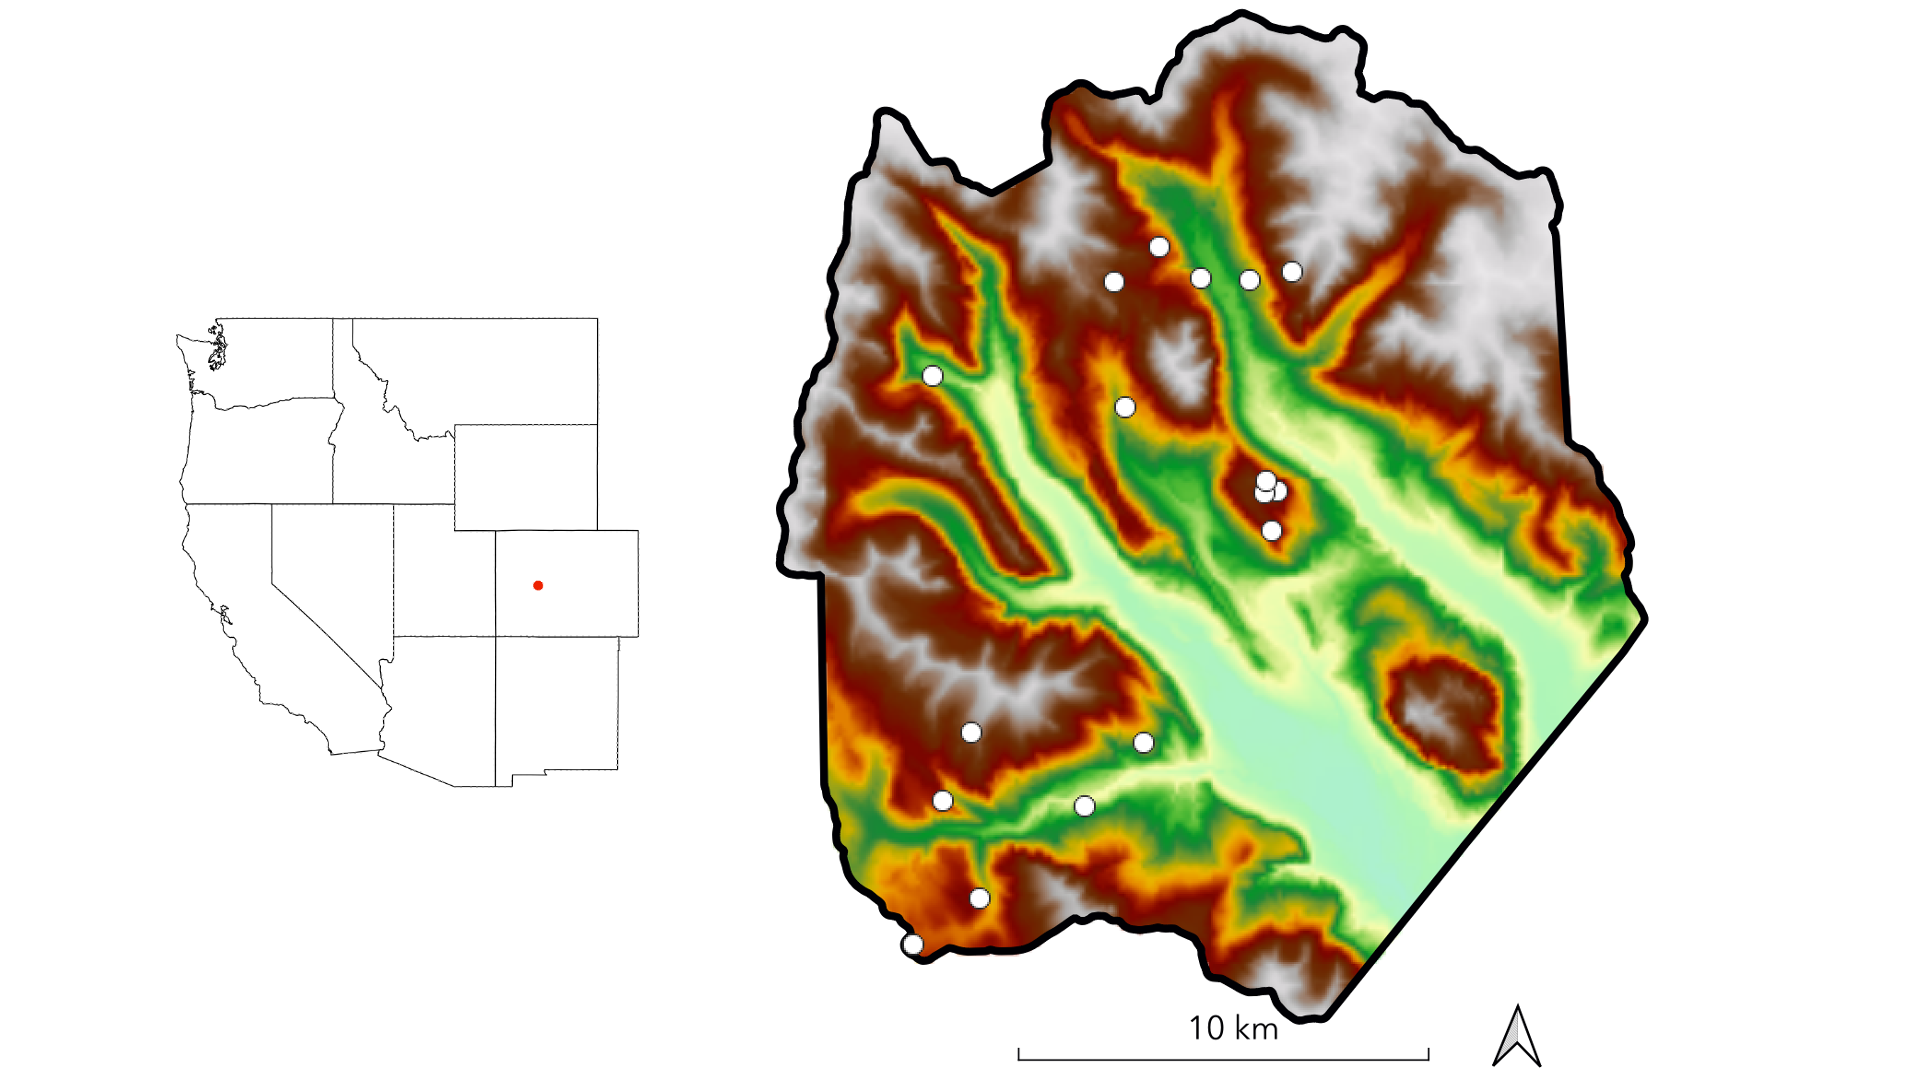
\includegraphics{./Figures/Fig1.png} \textbf{Figure 1.} The study domain
spans the footprint of a June 2018 NEON AOP acquisition in the East
River watershed in western Colorado. Dots indicate the locations of 0.16
ha conifer forest inventory plots. Shading is by elevation. \clearpage

\newpage

\subsection{Table 1}\label{table-1}

\textbf{Table 1.} Description and units of topographic variables used
for field plot selection.

\begin{longtable}[]{@{}
  >{\raggedright\arraybackslash}p{(\columnwidth - 4\tabcolsep) * \real{0.3333}}
  >{\raggedright\arraybackslash}p{(\columnwidth - 4\tabcolsep) * \real{0.4583}}
  >{\raggedright\arraybackslash}p{(\columnwidth - 4\tabcolsep) * \real{0.2083}}@{}}
\toprule\noalign{}
\begin{minipage}[b]{\linewidth}\raggedright
Variable
\end{minipage} & \begin{minipage}[b]{\linewidth}\raggedright
Description
\end{minipage} & \begin{minipage}[b]{\linewidth}\raggedright
Units
\end{minipage} \\
\midrule\noalign{}
\endhead
\bottomrule\noalign{}
\endlastfoot
Elevation & Elevation above sea level & m \\
Slope & dy/dx computed in a 30 m window & degrees \\
Folded aspect & Index of cardinal aspect adjusted for higher incident
radiation on SW slopes & unitless index \\
Heat load & Potential heat load calculated according to Eq. 3 in McCune
and Keon (2002) & unitless index \\
Topographic position index (1000 m) & Index of hillslope position
(summit, shoulder, backslope, footslope, and toeslope) computed in 1000
m window & unitless index \\
Topographic wetness index & Terrain-driven balance of upslope water
supply and local drainage (a function of local slope and upslope
contributing area per unit contour length) & unitless index \\
\end{longtable}

\clearpage

\newpage

\subsection{Table 2}\label{table-2}

\textbf{Table 2.} Measurements taken in field inventory with their units
and a summary of methods.

\begin{longtable}[]{@{}
  >{\raggedright\arraybackslash}p{(\columnwidth - 4\tabcolsep) * \real{0.5000}}
  >{\raggedright\arraybackslash}p{(\columnwidth - 4\tabcolsep) * \real{0.2273}}
  >{\raggedright\arraybackslash}p{(\columnwidth - 4\tabcolsep) * \real{0.2727}}@{}}
\toprule\noalign{}
\begin{minipage}[b]{\linewidth}\raggedright
Measurement
\end{minipage} & \begin{minipage}[b]{\linewidth}\raggedright
Units
\end{minipage} & \begin{minipage}[b]{\linewidth}\raggedright
Method
\end{minipage} \\
\midrule\noalign{}
\endhead
\bottomrule\noalign{}
\endlastfoot
Species & NA & Visual identification \\
Stem height & m & Nikon Forestry Pro II hypsometer, metric tape \\
DBH & cm & Diameter tape, calipers \\
Stem geolocation & decimal degrees & Trimble GEO-7X GPS unit held
against stem \\
Crown illumination & unitless index & Visual determination \\
Beetle damage & unitless index & Visual inspection for boreholes, sap,
red/grey needles \\
Life status & NA & Visual inspection for living/dead status \\
Health status & NA & Visual inspection for signs of infection, decay,
browning, wilting \\
\end{longtable}

\clearpage

\newpage

\subsection{Figure 2}\label{figure-2}

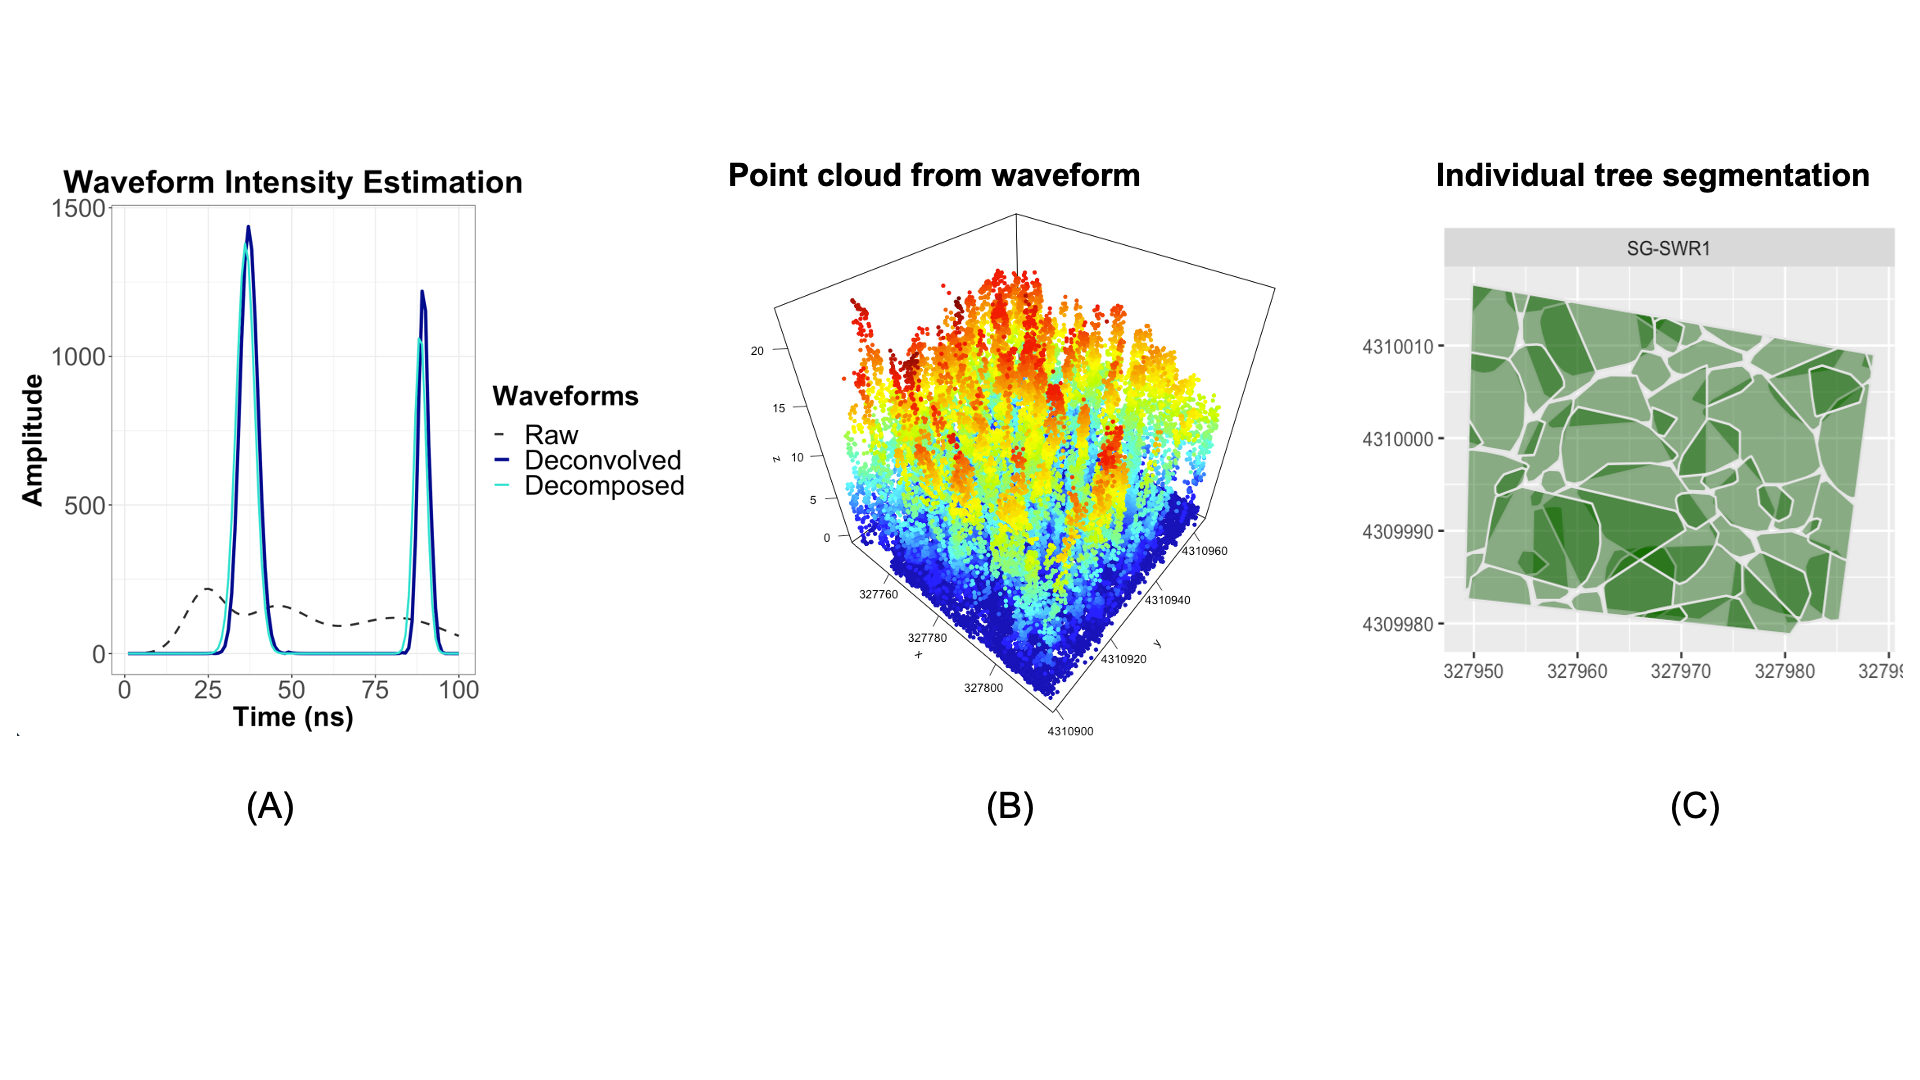
\includegraphics{./Figures/Fig2.png} \textbf{Figure 2.} Raw waveforms
were deconvolved with the outgoing ALS pulse and instrument impulse
response using the Gold algorithm, and then decomposed into a sum of
fitted Gaussian functions over time. Panel A shows the raw (dashed
black) waveform function and the resulting deconvolved (dark blue) and
decomposed (light blue) time series, all over a trimmed 100 ns support.
Waveform peaks and a random sample of values along peak slopes were
selected to generate a point cloud with a mean density of 24 points
\(m^-2\) across the acquisition area. An example of this high-density
point cloud at one inventory plot (SG-SWR1) with a 10 m buffer is shown
in panel B. The result of individual tree segmentation at the same plot,
with buffer removed, appears in panel C. \clearpage

\newpage

\subsection{Table 3}\label{table-3}

\textbf{Table 3.} Response (RE) and explanatory (EX) variables used in
statistical analysis.

\begin{Shaded}
\begin{Highlighting}[]
\FunctionTok{library}\NormalTok{(flextable)}
\NormalTok{v.type }\OtherTok{\textless{}{-}} \FunctionTok{c}\NormalTok{(}\FunctionTok{rep}\NormalTok{(}\StringTok{\textquotesingle{}Reponse\textquotesingle{}}\NormalTok{, }\DecValTok{5}\NormalTok{), }\FunctionTok{rep}\NormalTok{(}\StringTok{\textquotesingle{}Explanatory\textquotesingle{}}\NormalTok{, }\DecValTok{15}\NormalTok{))}
\NormalTok{v.name }\OtherTok{\textless{}{-}} \FunctionTok{c}\NormalTok{(}\StringTok{\textquotesingle{}Total number density\textquotesingle{}}\NormalTok{, }\StringTok{\textquotesingle{}QMD\textquotesingle{}}\NormalTok{, }
            \StringTok{\textquotesingle{}Basal area\textquotesingle{}}\NormalTok{, }\StringTok{\textquotesingle{}90th percentile height\textquotesingle{}}\NormalTok{, }\StringTok{\textquotesingle{}Height skew\textquotesingle{}}\NormalTok{, }\StringTok{\textquotesingle{}Elevation\textquotesingle{}}\NormalTok{,}
            \StringTok{\textquotesingle{}Slope\textquotesingle{}}\NormalTok{, }\StringTok{\textquotesingle{}Folded aspect\textquotesingle{}}\NormalTok{, }\StringTok{\textquotesingle{}Heat load\textquotesingle{}}\NormalTok{, }\StringTok{\textquotesingle{}TPI\textquotesingle{}}\NormalTok{, }\StringTok{\textquotesingle{}TWI\textquotesingle{}}\NormalTok{, }
            \StringTok{\textquotesingle{}AET\textquotesingle{}}\NormalTok{,}\StringTok{\textquotesingle{}CWD\textquotesingle{}}\NormalTok{,}\StringTok{\textquotesingle{}SWE\textquotesingle{}}\NormalTok{, }\StringTok{\textquotesingle{}∆SWE\textquotesingle{}}\NormalTok{, }\StringTok{\textquotesingle{}Available water capacity\textquotesingle{}}\NormalTok{, }
            \StringTok{\textquotesingle{}Organic matter\textquotesingle{}}\NormalTok{, }\StringTok{\textquotesingle{}k\textquotesingle{}}\NormalTok{, }\StringTok{\textquotesingle{}Total depth\textquotesingle{}}\NormalTok{, }\StringTok{\textquotesingle{}Lithologic substrate\textquotesingle{}}\NormalTok{)}
\NormalTok{v.desc }\OtherTok{\textless{}{-}} \FunctionTok{c}\NormalTok{(}\StringTok{\textquotesingle{}Total number of ITC objects per grid cell\textquotesingle{}}\NormalTok{,}
            \StringTok{\textquotesingle{}Quadratic mean of stem diameters of objects per grid cell\textquotesingle{}}\NormalTok{,}
            \StringTok{\textquotesingle{}Sum of cross{-}sectional areas of stems per hectare\textquotesingle{}}\NormalTok{,}
            \StringTok{\textquotesingle{}Estimated maximum canopy height per grid cell\textquotesingle{}}\NormalTok{,}
            \StringTok{\textquotesingle{}Third moment of height distribution per grid cell\textquotesingle{}}\NormalTok{,}
            \StringTok{\textquotesingle{}Elevation above sea level\textquotesingle{}}\NormalTok{,}
            \StringTok{\textquotesingle{}dz/dxy computed in a 30 m window\textquotesingle{}}\NormalTok{,}
            \StringTok{\textquotesingle{}Index of cardinal aspect adjusted for higher incident radiation on SW slopes\textquotesingle{}}\NormalTok{,}
            \StringTok{\textquotesingle{}Potential heat load calculated according to Eq. 3 in McCune and Keon (2002)\textquotesingle{}}\NormalTok{,}
            \StringTok{\textquotesingle{}Index of hillslope position (summit, shoulder, backslope, footslope, and toeslope) computed in 1000 m window\textquotesingle{}}\NormalTok{,}
            \StringTok{\textquotesingle{}Terrain{-}driven ratio of upslope water supply to local drainage expressed as afunction of local slope and upslope contributing area per unit contour length, computed on a 100 m pixel scale\textquotesingle{}}\NormalTok{,}
            \StringTok{\textquotesingle{}Actual evapotranspiration: depth of water (mm) evaporated from the surface or transpired by plants per grid cell\textquotesingle{}}\NormalTok{,}
            \StringTok{\textquotesingle{}Climatic water deficit: difference between potential evapotranspiration (PET) and AET, where PET is the total depth of water that can be evaporated or transpired given prevailing atmospheric conditions\textquotesingle{}}\NormalTok{,}
            \StringTok{\textquotesingle{}Snow water equivalent derived by forcing iSnobal with 50 m snow depth data from eight Airborne Snow Observatory flights\textquotesingle{}}\NormalTok{,}
            \StringTok{\textquotesingle{}Relative velocity of snow disappearance; difference between winter SWE and summer SWE divided by days between flights averaged over three flight{-}years\textquotesingle{}}\NormalTok{,}
            \StringTok{\textquotesingle{}Amount of plant{-}available water that can be stored in a unit of soil depth\textquotesingle{}}\NormalTok{,}
            \StringTok{\textquotesingle{}Amount of decomposed plant and animal residue expressed as a weight percentage of the less than 2 mm soil material\textquotesingle{}}\NormalTok{,}
            \StringTok{\textquotesingle{}Amount of water that moves vertically through a unit area of soil per unit time under unit hydraulic gradient\textquotesingle{}}\NormalTok{,}
            \StringTok{\textquotesingle{}Sum of horizon depths in a soil component\textquotesingle{}}\NormalTok{,}
            \StringTok{\textquotesingle{}Distribution of rock formations\textquotesingle{}}
\NormalTok{            )}

\NormalTok{v.cat }\OtherTok{\textless{}{-}} \FunctionTok{c}\NormalTok{(}\FunctionTok{rep}\NormalTok{(}\StringTok{\textquotesingle{}Forest structure\textquotesingle{}}\NormalTok{, }\DecValTok{5}\NormalTok{),}
             \FunctionTok{rep}\NormalTok{(}\StringTok{\textquotesingle{}Topography\textquotesingle{}}\NormalTok{, }\DecValTok{6}\NormalTok{),}
             \FunctionTok{rep}\NormalTok{(}\StringTok{\textquotesingle{}Climate\textquotesingle{}}\NormalTok{, }\DecValTok{4}\NormalTok{),}
             \FunctionTok{rep}\NormalTok{(}\StringTok{\textquotesingle{}Soil\textquotesingle{}}\NormalTok{, }\DecValTok{4}\NormalTok{),}
             \StringTok{\textquotesingle{}Geology\textquotesingle{}}
\NormalTok{             )}

\NormalTok{v.unit }\OtherTok{\textless{}{-}} \FunctionTok{c}\NormalTok{(}\StringTok{\textquotesingle{}stems ha\^{}{-}1\textquotesingle{}}\NormalTok{, }\StringTok{\textquotesingle{}cm\textquotesingle{}}\NormalTok{, }\StringTok{\textquotesingle{}m\^{}2\textquotesingle{}}\NormalTok{, }\StringTok{\textquotesingle{}m\textquotesingle{}}\NormalTok{, }\StringTok{\textquotesingle{}NA\textquotesingle{}}\NormalTok{,}
            \StringTok{\textquotesingle{}m\textquotesingle{}}\NormalTok{, }\StringTok{\textquotesingle{}degrees\textquotesingle{}}\NormalTok{, }\StringTok{\textquotesingle{}index\textquotesingle{}}\NormalTok{, }\StringTok{\textquotesingle{}index\textquotesingle{}}\NormalTok{, }\StringTok{\textquotesingle{}index\textquotesingle{}}\NormalTok{, }\StringTok{\textquotesingle{}index\textquotesingle{}}\NormalTok{,}
            \StringTok{\textquotesingle{}m\textquotesingle{}}\NormalTok{, }\StringTok{\textquotesingle{}m day\^{}{-}1\textquotesingle{}}\NormalTok{, }\StringTok{\textquotesingle{}mm\textquotesingle{}}\NormalTok{, }\StringTok{\textquotesingle{}mm\textquotesingle{}}\NormalTok{,}
            \StringTok{\textquotesingle{}mm\textquotesingle{}}\NormalTok{, }\StringTok{\textquotesingle{}\% mass\textquotesingle{}}\NormalTok{, }\StringTok{\textquotesingle{}μm sec\^{}{-}1\textquotesingle{}}\NormalTok{, }\StringTok{\textquotesingle{}cm\textquotesingle{}}\NormalTok{, }
            \StringTok{\textquotesingle{}NA\textquotesingle{}}\NormalTok{)}

\NormalTok{v.src }\OtherTok{\textless{}{-}} \FunctionTok{c}\NormalTok{(}\FunctionTok{rep}\NormalTok{(}\StringTok{\textquotesingle{}NEON LiDAR\textquotesingle{}}\NormalTok{, }\DecValTok{5}\NormalTok{),}
           \FunctionTok{rep}\NormalTok{(}\StringTok{\textquotesingle{}NEON LiDAR\textquotesingle{}}\NormalTok{, }\DecValTok{6}\NormalTok{),}
           \FunctionTok{rep}\NormalTok{(}\StringTok{\textquotesingle{}BCM (Budo et al. 2017)\textquotesingle{}}\NormalTok{, }\DecValTok{2}\NormalTok{), }\FunctionTok{rep}\NormalTok{(}\StringTok{\textquotesingle{}ASO\textquotesingle{}}\NormalTok{, }\DecValTok{2}\NormalTok{),}
           \FunctionTok{rep}\NormalTok{(}\StringTok{\textquotesingle{}SSURGO\textquotesingle{}}\NormalTok{, }\DecValTok{4}\NormalTok{),}
           \StringTok{\textquotesingle{}Colorado Geological Survey\textquotesingle{}}\NormalTok{)}

\NormalTok{var.tbl }\OtherTok{\textless{}{-}} \FunctionTok{data.frame}\NormalTok{(}\FunctionTok{cbind}\NormalTok{(}\StringTok{\textquotesingle{}Type\textquotesingle{}}\OtherTok{=}\NormalTok{v.type, }\StringTok{\textquotesingle{}Category\textquotesingle{}}\OtherTok{=}\NormalTok{v.cat, }
                            \StringTok{\textquotesingle{}Variable\textquotesingle{}}\OtherTok{=}\NormalTok{v.name, }\StringTok{\textquotesingle{}Description\textquotesingle{}}\OtherTok{=}\NormalTok{v.desc, }
                            \StringTok{\textquotesingle{}Units\textquotesingle{}}\OtherTok{=}\NormalTok{v.unit, }\StringTok{\textquotesingle{}Source\textquotesingle{}}\OtherTok{=}\NormalTok{v.src))}

\NormalTok{ft }\OtherTok{\textless{}{-}} \FunctionTok{flextable}\NormalTok{(var.tbl)}
\end{Highlighting}
\end{Shaded}

\clearpage

\newpage

\subsection{Table 4}\label{table-4}

\textbf{Table 4.} Summary statistics for the best-performing runs of six
individual tree delineation (ITD) algorithms. Parameters and values for
each run appear in Supplementary Material. Averages and standard
deviations were taken for results across plots.

\begin{longtable}[]{@{}
  >{\raggedright\arraybackslash}p{(\columnwidth - 24\tabcolsep) * \real{0.0360}}
  >{\raggedright\arraybackslash}p{(\columnwidth - 24\tabcolsep) * \real{0.0216}}
  >{\raggedright\arraybackslash}p{(\columnwidth - 24\tabcolsep) * \real{0.1439}}
  >{\raggedright\arraybackslash}p{(\columnwidth - 24\tabcolsep) * \real{0.1367}}
  >{\raggedright\arraybackslash}p{(\columnwidth - 24\tabcolsep) * \real{0.1079}}
  >{\raggedright\arraybackslash}p{(\columnwidth - 24\tabcolsep) * \real{0.1007}}
  >{\raggedright\arraybackslash}p{(\columnwidth - 24\tabcolsep) * \real{0.0719}}
  >{\raggedright\arraybackslash}p{(\columnwidth - 24\tabcolsep) * \real{0.1151}}
  >{\raggedright\arraybackslash}p{(\columnwidth - 24\tabcolsep) * \real{0.0647}}
  >{\raggedright\arraybackslash}p{(\columnwidth - 24\tabcolsep) * \real{0.0791}}
  >{\raggedright\arraybackslash}p{(\columnwidth - 24\tabcolsep) * \real{0.0647}}
  >{\raggedright\arraybackslash}p{(\columnwidth - 24\tabcolsep) * \real{0.0432}}
  >{\raggedright\arraybackslash}p{(\columnwidth - 24\tabcolsep) * \real{0.0144}}@{}}
\toprule\noalign{}
\begin{minipage}[b]{\linewidth}\raggedright
Model
\end{minipage} & \begin{minipage}[b]{\linewidth}\raggedright
Run
\end{minipage} & \begin{minipage}[b]{\linewidth}\raggedright
Total observed trees
\end{minipage} & \begin{minipage}[b]{\linewidth}\raggedright
Total modeled trees
\end{minipage} & \begin{minipage}[b]{\linewidth}\raggedright
Mean (s.d.) extraction rate
\end{minipage} & \begin{minipage}[b]{\linewidth}\raggedright
Mean (s.d.) match rate
\end{minipage} & \begin{minipage}[b]{\linewidth}\raggedright
Mean (s.d.) accuracy
\end{minipage} & \begin{minipage}[b]{\linewidth}\raggedright
Omissions
\end{minipage} & \begin{minipage}[b]{\linewidth}\raggedright
Commissions
\end{minipage} & \begin{minipage}[b]{\linewidth}\raggedright
Precision
\end{minipage} & \begin{minipage}[b]{\linewidth}\raggedright
Recall
\end{minipage} & \begin{minipage}[b]{\linewidth}\raggedright
f
\end{minipage} & \begin{minipage}[b]{\linewidth}\raggedright
\end{minipage} \\
\midrule\noalign{}
\endhead
\bottomrule\noalign{}
\endlastfoot
LayerStacking & 11 & 4303 & 4274 & 1.11 (0.37) & 0.51 (0.11) & 0.53
(0.10) & 0.10 & 0.11 & 0.51 (0.11) & 0.54 (0.10) & 0.51 (0.05) & \\
\end{longtable}

\subsection{Table 5}\label{table-5}

\textbf{Table 5.} Root mean squared difference in horizontal and
vertical dimensions between field-observed and modeled trees for the
best-performing runs of each ITD model tested.

\begin{longtable}[]{@{}lllll@{}}
\toprule\noalign{}
Model & Run & RMSE\_\{xy\} (m) & RMSE\_\{z\} (m) & Loss \\
\midrule\noalign{}
\endhead
\bottomrule\noalign{}
\endlastfoot
LayerStacking & 11 & 2.59 & 1.59 & 6.09 \\
PTrees & & & & \\
& & & & \\
\end{longtable}

\clearpage

\newpage

\subsection{Figure 3}\label{figure-3}

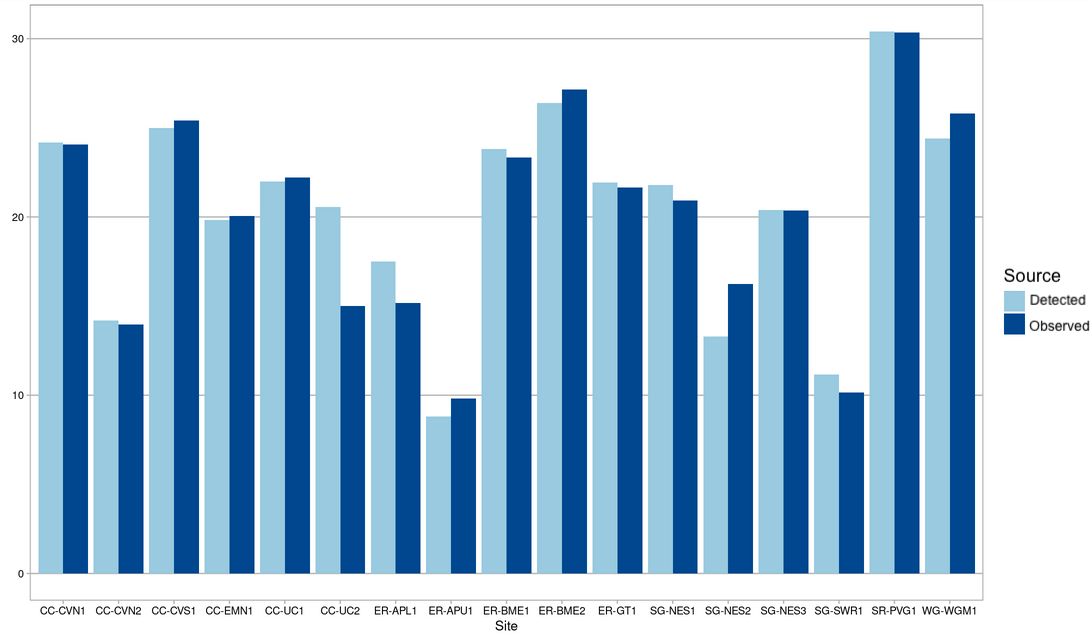
\includegraphics{./Figures/Fig3.png} \textbf{Figure 3.} Diameter and
height distributions of trees measured in inventory plots across all
sites (A), and by species (B, C).

\clearpage

\newpage

\subsection{Figure 4}\label{figure-4}

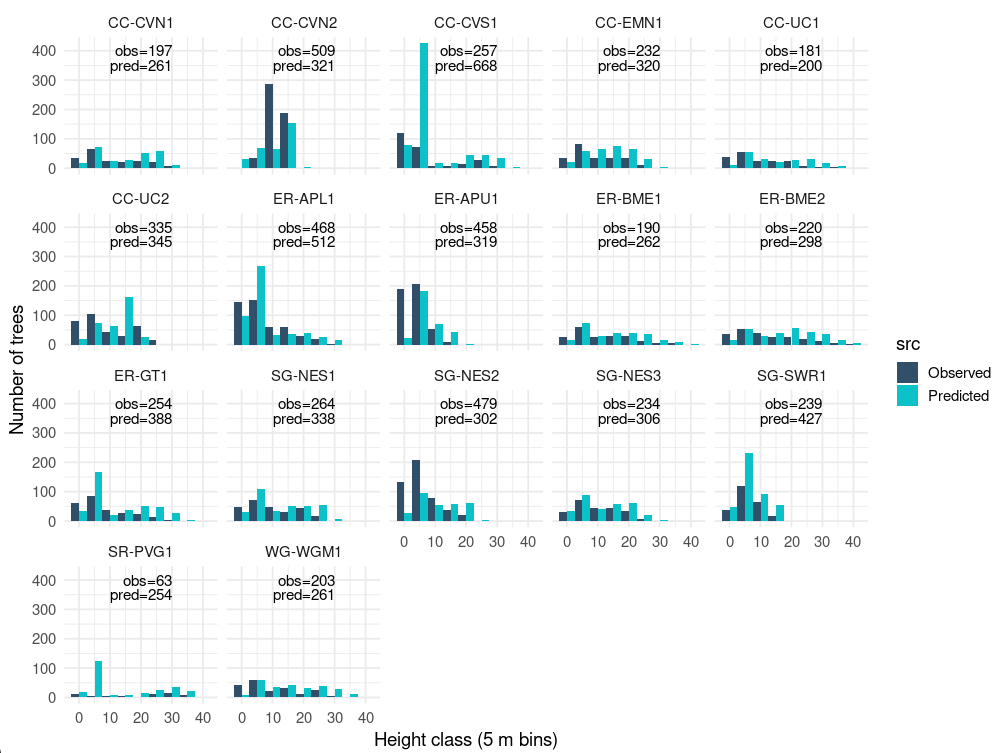
\includegraphics{./Figures/Fig4.png} \textbf{Figure 4.} Total number of
trees measured in plots (``Observed''---dark blue) and detected in
segmentation of the ALS point cloud (``Predicted''---light blue), by
height class, in 1 m increments. \clearpage

\newpage

\subsection{Figure 5}\label{figure-5}

{[}TODO - comparison of modeled QMD and field QMD in plots{]}

\subsection{Figure 6}\label{figure-6}

{[}TODO - frequency distribution of heights and diameters of modeled
trees{]}

\subsection{Figure 7}\label{figure-7}

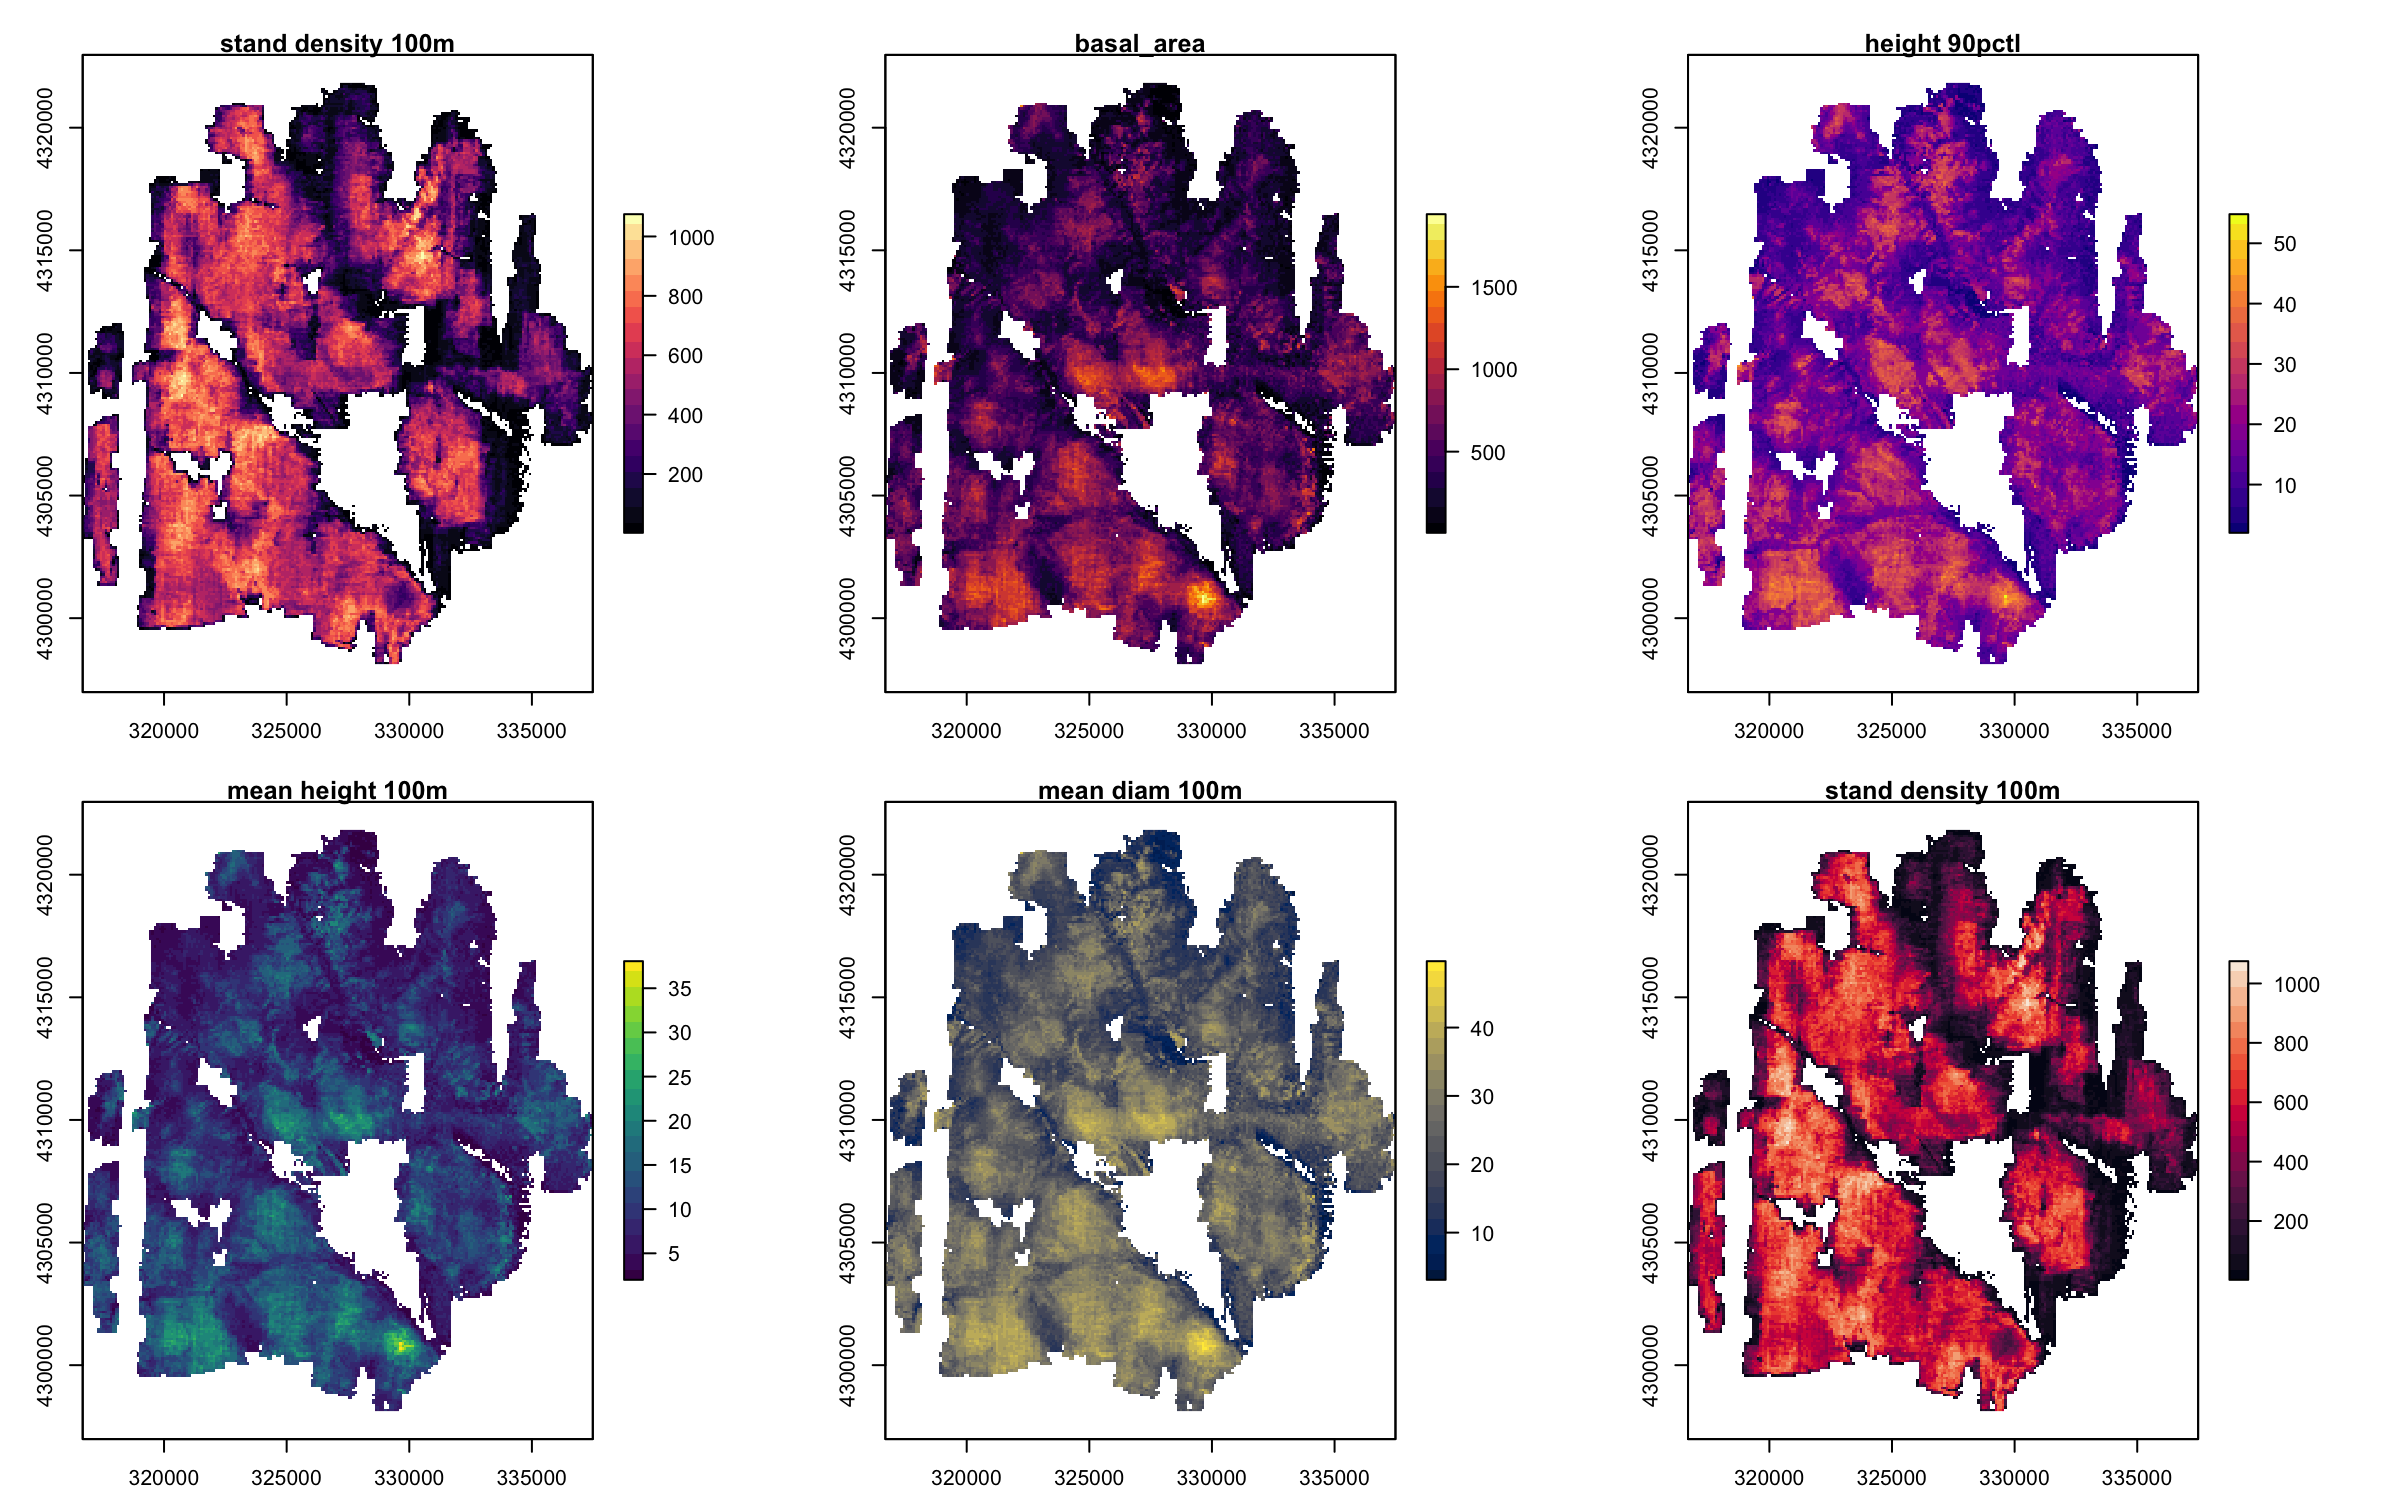
\includegraphics{./Figures/Fig5.png} \textbf{Figure 7.} Maps of forest
structure metrics at 100 m grid resolution. \clearpage

\newpage

\subsection{Figure 8}\label{figure-8}

{[}TODO - state factor maps{]}

\subsection{Table 4. Summary statistics by species for trees observed in
field
census.}\label{table-4.-summary-statistics-by-species-for-trees-observed-in-field-census.}

\begin{longtable}[]{@{}
  >{\raggedright\arraybackslash}p{(\columnwidth - 10\tabcolsep) * \real{0.0825}}
  >{\raggedleft\arraybackslash}p{(\columnwidth - 10\tabcolsep) * \real{0.0515}}
  >{\raggedleft\arraybackslash}p{(\columnwidth - 10\tabcolsep) * \real{0.1856}}
  >{\raggedleft\arraybackslash}p{(\columnwidth - 10\tabcolsep) * \real{0.1649}}
  >{\raggedleft\arraybackslash}p{(\columnwidth - 10\tabcolsep) * \real{0.2784}}
  >{\raggedleft\arraybackslash}p{(\columnwidth - 10\tabcolsep) * \real{0.2371}}@{}}
\toprule\noalign{}
\begin{minipage}[b]{\linewidth}\raggedright
Sp\_Code
\end{minipage} & \begin{minipage}[b]{\linewidth}\raggedleft
N
\end{minipage} & \begin{minipage}[b]{\linewidth}\raggedleft
Median height (m)
\end{minipage} & \begin{minipage}[b]{\linewidth}\raggedleft
Median DBH (cm)
\end{minipage} & \begin{minipage}[b]{\linewidth}\raggedleft
Stem Density (stems ha\^{}-1)
\end{minipage} & \begin{minipage}[b]{\linewidth}\raggedleft
Basal area (m\^{}2 ha\^{}-1)
\end{minipage} \\
\midrule\noalign{}
\endhead
\bottomrule\noalign{}
\endlastfoot
ABLA & 3464 & 4 & 5.6 & 1274 & 17.8 \\
PICO & 676 & 12 & 13.8 & 249 & 6.2 \\
PIEN & 1574 & 8 & 11.7 & 579 & 25.9 \\
POTR & 37 & 5 & 8.2 & 14 & 0.1 \\
\end{longtable}

\subsection{Table 5. Summary statistics by plot for trees observed in
field
census.}\label{table-5.-summary-statistics-by-plot-for-trees-observed-in-field-census.}

\begin{longtable}[]{@{}
  >{\raggedright\arraybackslash}p{(\columnwidth - 12\tabcolsep) * \real{0.1064}}
  >{\raggedleft\arraybackslash}p{(\columnwidth - 12\tabcolsep) * \real{0.0426}}
  >{\raggedleft\arraybackslash}p{(\columnwidth - 12\tabcolsep) * \real{0.1064}}
  >{\raggedleft\arraybackslash}p{(\columnwidth - 12\tabcolsep) * \real{0.1915}}
  >{\raggedleft\arraybackslash}p{(\columnwidth - 12\tabcolsep) * \real{0.1702}}
  >{\raggedleft\arraybackslash}p{(\columnwidth - 12\tabcolsep) * \real{0.1383}}
  >{\raggedleft\arraybackslash}p{(\columnwidth - 12\tabcolsep) * \real{0.2447}}@{}}
\toprule\noalign{}
\begin{minipage}[b]{\linewidth}\raggedright
Site\_Name
\end{minipage} & \begin{minipage}[b]{\linewidth}\raggedleft
N
\end{minipage} & \begin{minipage}[b]{\linewidth}\raggedleft
N species
\end{minipage} & \begin{minipage}[b]{\linewidth}\raggedleft
Median height (m)
\end{minipage} & \begin{minipage}[b]{\linewidth}\raggedleft
Median DBH (cm)
\end{minipage} & \begin{minipage}[b]{\linewidth}\raggedleft
Stem Density
\end{minipage} & \begin{minipage}[b]{\linewidth}\raggedleft
Basal area (m\^{}2 ha\^{}-1)
\end{minipage} \\
\midrule\noalign{}
\endhead
\bottomrule\noalign{}
\endlastfoot
CC-CVN1 & 224 & 2 & 5 & 9.8 & 1400 & 49.0 \\
CC-CVN2 & 526 & 3 & 12 & 12.2 & 3288 & 47.5 \\
CC-CVS1 & 326 & 2 & 2 & 2.5 & 2038 & 34.1 \\
CC-EMN1 & 294 & 2 & 5 & 8.9 & 1838 & 61.8 \\
CC-UC1 & 199 & 2 & 7 & 11.7 & 1244 & 49.3 \\
CC-UC2 & 335 & 2 & 6 & 9.1 & 2094 & 53.0 \\
ER-APL1 & 494 & 2 & 4 & 5.9 & 3088 & 65.7 \\
ER-APU1 & 471 & 2 & 3 & 4.9 & 2944 & 27.1 \\
ER-BME1 & 197 & 2 & 10 & 15.3 & 1231 & 62.3 \\
ER-BME2 & 220 & 2 & 9 & 11.9 & 1375 & 54.5 \\
ER-GT1 & 278 & 2 & 6 & 8.2 & 1738 & 46.1 \\
SG-NES1 & 478 & 3 & 3 & 5.2 & 2988 & 54.3 \\
SG-NES2 & 488 & 3 & 4 & 5.8 & 3050 & 43.1 \\
SG-NES3 & 399 & 3 & 4 & 5.9 & 2494 & 44.9 \\
SG-SWR1 & 287 & 4 & 5 & 9.1 & 1794 & 30.7 \\
SR-PVG1 & 66 & 2 & 23 & 32.7 & 412 & 40.8 \\
WG-WGM1 & 209 & 2 & 7 & 10.5 & 1306 & 50.2 \\
XX-CAR3 & 260 & 4 & 8 & 10.7 & 1625 & 34.6 \\
\end{longtable}

\subsection{Figure 9}\label{figure-9}

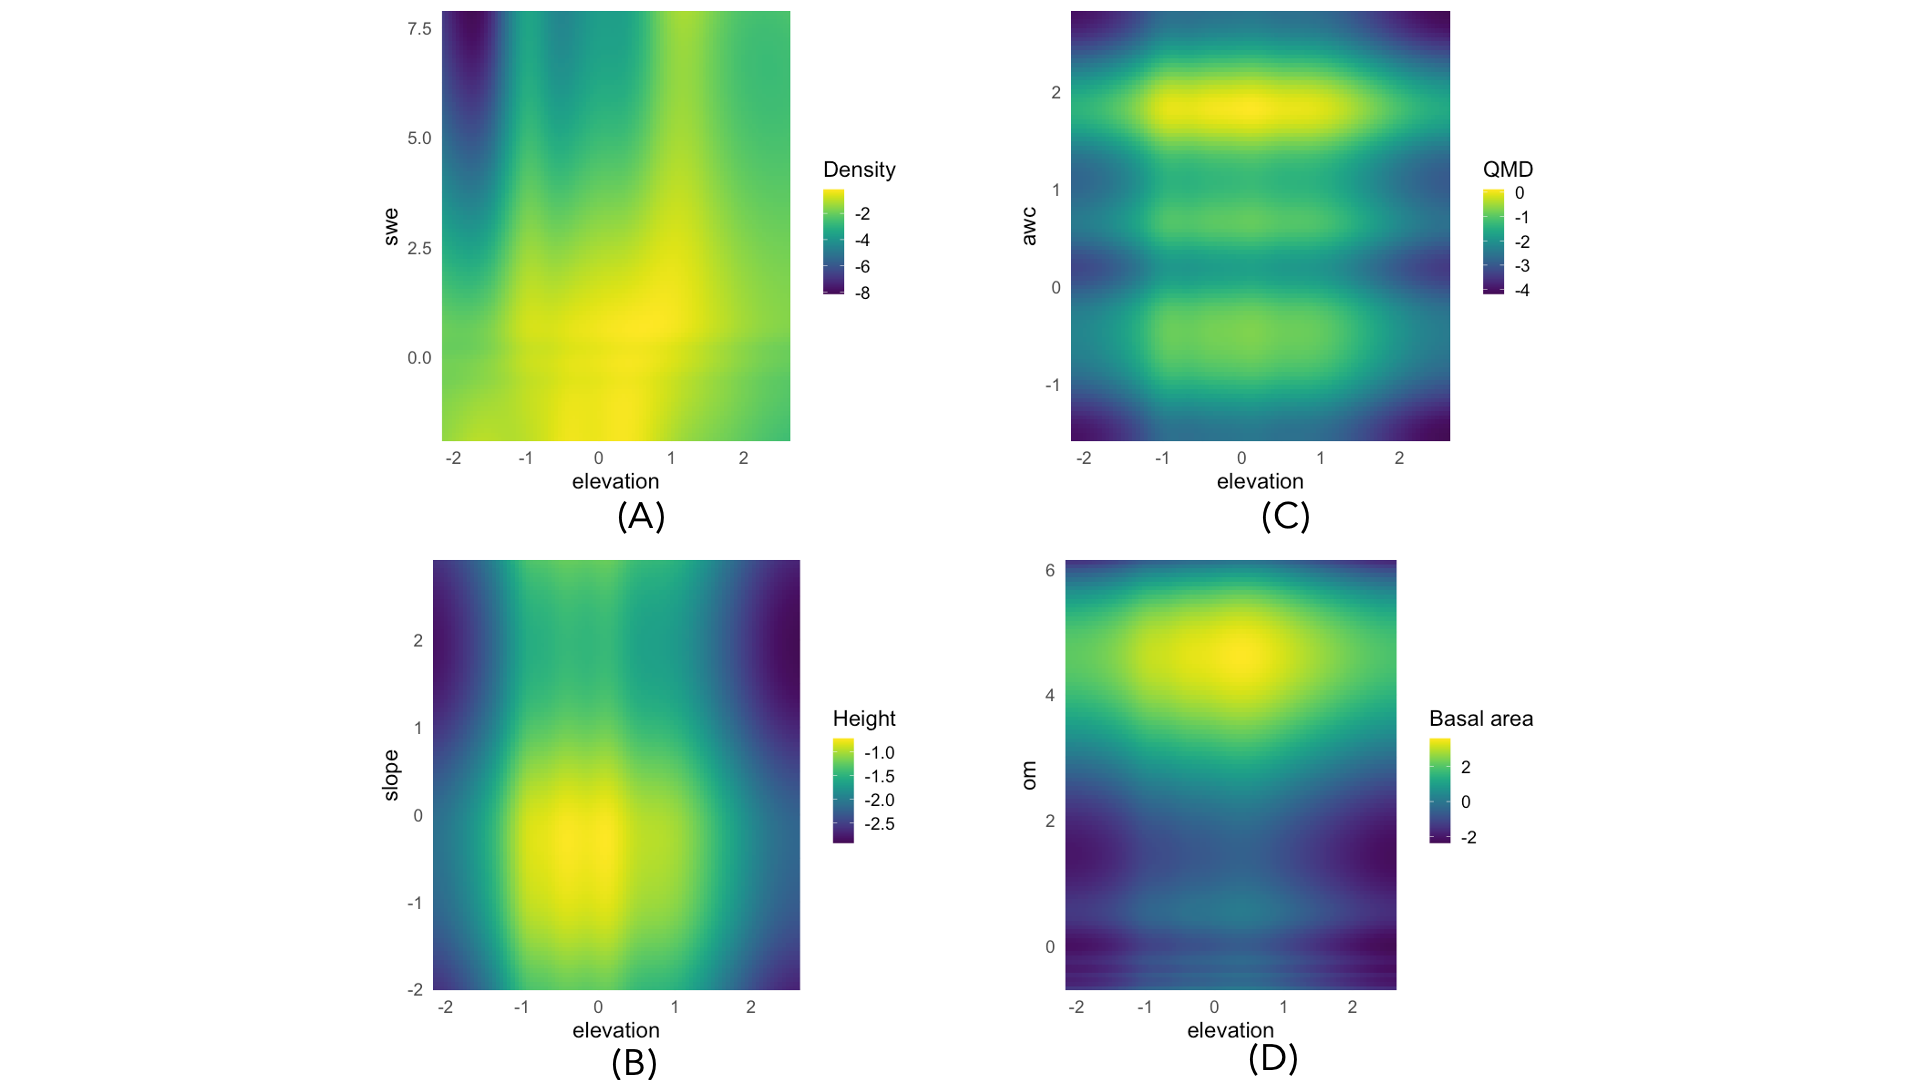
\includegraphics{./Figures/Fig6.png} \textbf{Figure 9.} Variable
interaction plots demonstrate the strong, nonlinear elevational control
on density (A), 90th percentile height (B), QMD (C), and basal area (D).
Interaction plots show the two strongest explainers of each response
variable. The influence of elevation is mediated by SWE, slope angle,
soil AWC, and soil organic matter, respectively. \clearpage

\newpage

\subsection{Figure 10}\label{figure-10}

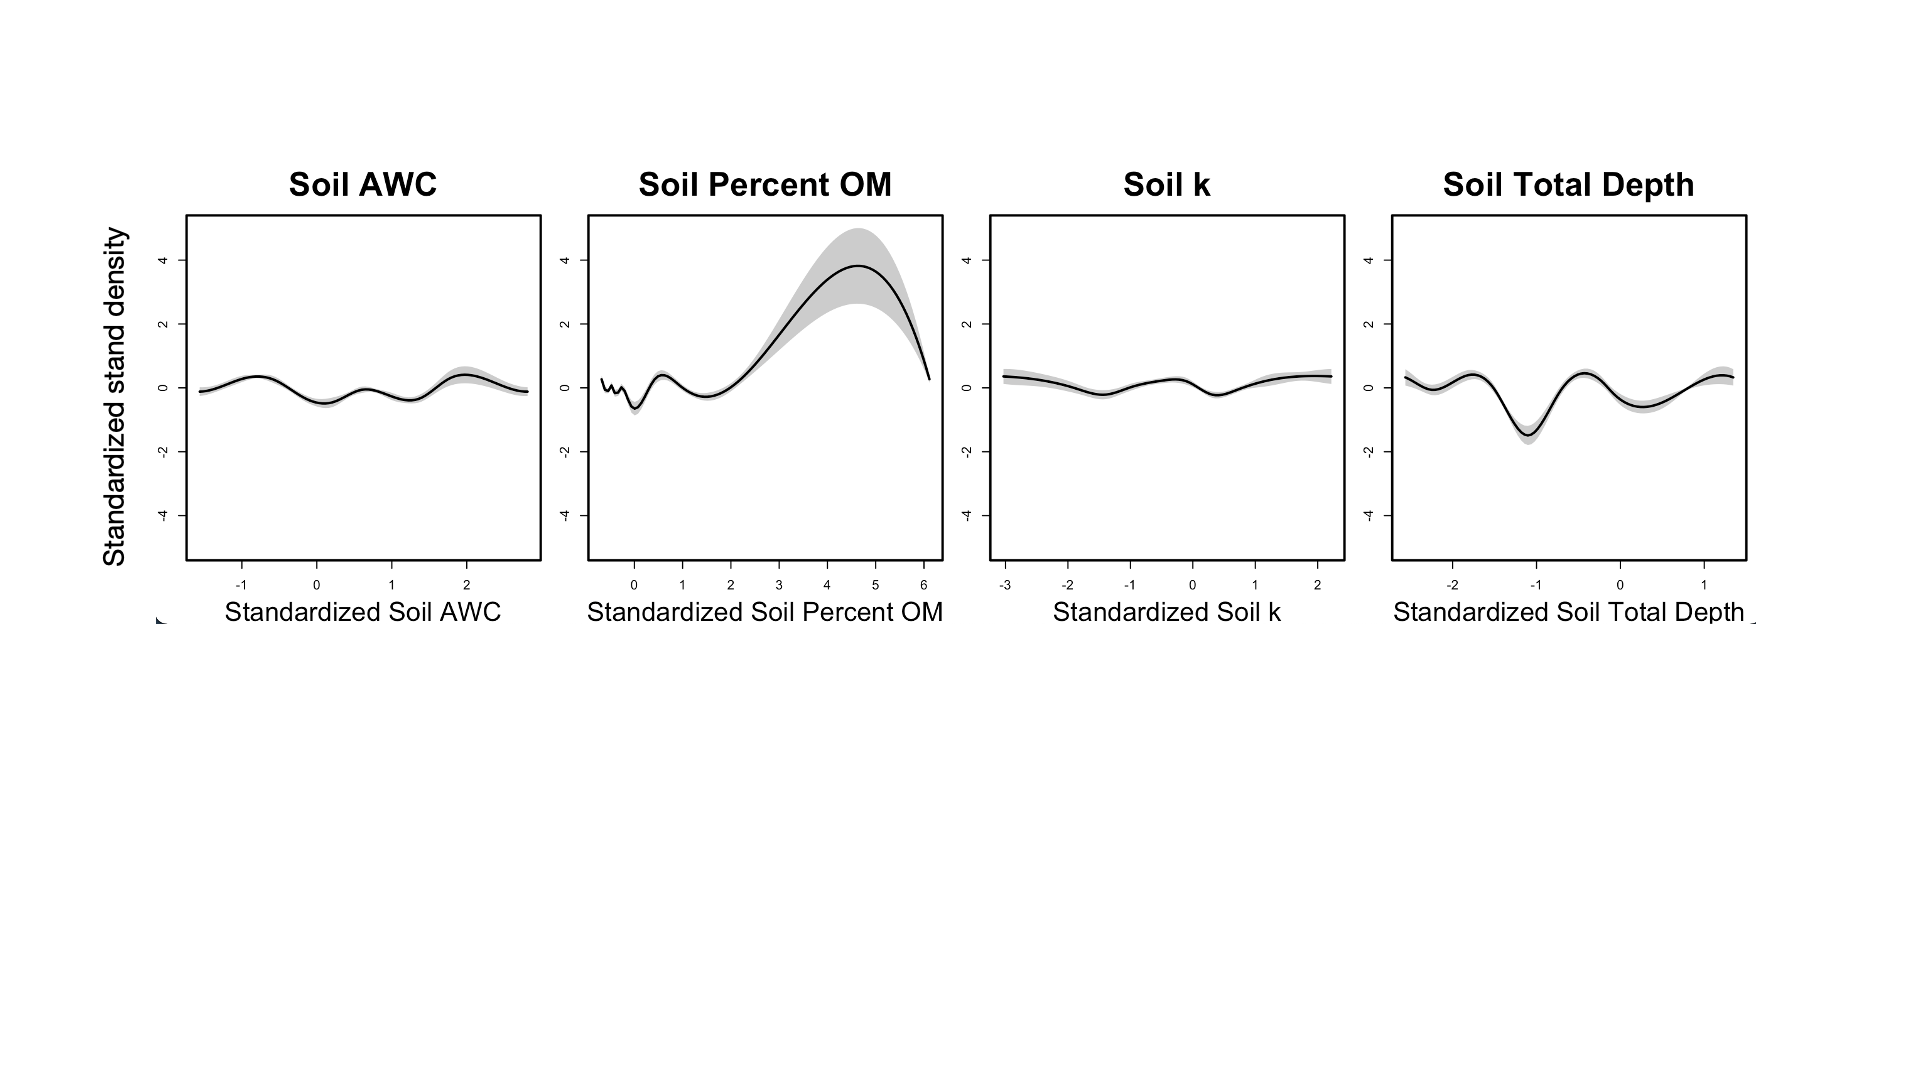
\includegraphics{./Figures/Fig7.png} \textbf{Figure 10.} Stand density
increased with soil organic matter and was at minimum with soil total
depth = 50 cm, but other soil properties had little correlation with
stand density. \clearpage

\newpage

\section{Supplementary Materials}\label{supplementary-materials}

\section*{References}\label{references}
\addcontentsline{toc}{section}{References}

\phantomsection\label{refs}
\setlength{\cslentryspacing}{0em}
\begin{CSLReferences}
\bibitem[\citeproctext]{ref-amundson_state_1997}
Amundson, R., Jenny, H., 1997. On a {State} {Factor} {Model} of
{Ecosystems}. BioScience 47, 536--543.
\url{https://doi.org/10.2307/1313122}

\bibitem[\citeproctext]{ref-bolstad_forests_2018}
Bolstad, P.V., Elliott, K.J., Miniat, C.F., 2018. Forests, shrubs, and
terrain: Top‐down and bottom‐up controls on forest structure. Ecosphere
9. \url{https://doi.org/10.1002/ecs2.2185}

\bibitem[\citeproctext]{ref-dalponte_tree-centric_2016}
Dalponte, M., Coomes, D.A., 2016. Tree-centric mapping of forest carbon
density from airborne laser scanning and hyperspectral data. Methods in
Ecology and Evolution 7, 1236--1245.
\url{https://doi.org/10.1111/2041-210X.12575}

\bibitem[\citeproctext]{ref-jenny_derivation_1961}
Jenny, H., 1961. Derivation of {State} {Factor} {Equations} of {Soils}
and {Ecosystems}. Soil Science Society of America Journal 25, 385--388.
\url{https://doi.org/10.2136/sssaj1961.03615995002500050023x}

\bibitem[\citeproctext]{ref-kane_water_2015}
Kane, V.R., Lutz, J.A., Alina Cansler, C., Povak, N.A., Churchill, D.J.,
Smith, D.F., Kane, J.T., North, M.P., 2015. Water balance and topography
predict fire and forest structure patterns. Forest Ecology and
Management 338, 1--13.
\url{https://doi.org/10.1016/j.foreco.2014.10.038}

\bibitem[\citeproctext]{ref-lookingbill_empirical_2004}
Lookingbill, T., Urban, D., 2004. An empirical approach towards improved
spatial estimates of soil moisture for vegetation analysis. Landscape
Ecology 19, 417--433.
\url{https://doi.org/10.1023/B:LAND.0000030451.29571.8b}

\bibitem[\citeproctext]{ref-lydersen_topographic_2012}
Lydersen, J., North, M., 2012. Topographic {Variation} in {Structure} of
{Mixed}-{Conifer} {Forests} {Under} an {Active}-{Fire} {Regime}.
Ecosystems 15, 1134--1146.
\url{https://doi.org/10.1007/s10021-012-9573-8}

\bibitem[\citeproctext]{ref-mcnab_topographic_1993}
McNab, W.H., 1993. A topographic index to quantify the effect of
mesoscale landform on site productivity. Canadian Journal of Forest
Research 23, 1100--1107. \url{https://doi.org/10.1139/x93-140}

\bibitem[\citeproctext]{ref-mcnab_terrain_1989}
McNab, W.H., 1989. Terrain {Shape} {Index}: {Quantifying} {Effect} of
{Minor} {Landforms} on {Tree} {Height}. Forest Science 35, 91--104.
\url{https://doi.org/10.1093/forestscience/35.1.91}

\end{CSLReferences}

\end{document}
